%====================================================
% UNIVERSITY OF ECONOMICS HO CHI MINH CITY (UEH)
% GRADUATE ACADEMIC TEMPLATE 
%====================================================

\documentclass[12pt,a4paper]{article}

%----------------------------------------------------
% COLOR THEME (UEH)
%----------------------------------------------------
\usepackage{xcolor}
\definecolor{uehblue}{RGB}{0,70,127}
\definecolor{uehgray}{RGB}{80,80,80}

%----------------------------------------------------
% LANGUAGE & FONT (Requires XeLaTeX or LuaLaTeX)
%----------------------------------------------------
\usepackage{polyglossia}
\setmainlanguage{vietnamese}
\usepackage{fontspec}
\setmainfont{Times New Roman}

% Việt hóa tự động các tiêu đề danh mục
\addto\captionsvietnamese{
	\renewcommand{\contentsname}{Mục lục}
	\renewcommand{\listfigurename}{Danh mục hình vẽ}
	\renewcommand{\listtablename}{Danh mục bảng biểu}
}

%----------------------------------------------------
% PAGE LAYOUT
%----------------------------------------------------
\usepackage{geometry}
\geometry{
	left=3cm,
	right=2cm,
	top=2.5cm,
	bottom=3cm
}

\usepackage{setspace}
\onehalfspacing % Giãn dòng 1.5

\setlength{\parindent}{0pt}
\setlength{\parskip}{6pt}

% FIX HEADER HEIGHT
\setlength{\headheight}{14.5pt}

%----------------------------------------------------
% CORE PACKAGES
%----------------------------------------------------
\usepackage{graphicx}
\graphicspath{{figures/}} % Lưu hình ảnh vào thư mục figures/
\usepackage{subcaption}
\usepackage{float}

% Table packages
\usepackage{booktabs}
\usepackage{longtable}
\usepackage{array}
\usepackage{threeparttable}

% Math packages
\usepackage{amsmath,amssymb}

% TOC formatting
\usepackage{tocloft}
\usepackage{etoolbox}
\usepackage{afterpage}

%----------------------------------------------------
% FIGURE & TABLE CAPTION
%----------------------------------------------------
\usepackage{caption}
\captionsetup{
	font=small,
	labelfont=bf,
	justification=raggedright,
	singlelinecheck=false
}

%----------------------------------------------------
% HYPERLINKS
%----------------------------------------------------
\usepackage{hyperref}
\hypersetup{
	colorlinks=true,
	linkcolor=black,
	citecolor=uehblue,
	urlcolor=uehblue
}

%----------------------------------------------------
% HEADER & FOOTER – UEH
%----------------------------------------------------
\usepackage{fancyhdr}
\usepackage{lastpage}
\pagestyle{fancy}
\fancyhf{}

% Header
\fancyhead[L]{\small\textit{Đại học Kinh tế Thành phố Hồ Chí Minh}}
\fancyhead[R]{\small\textit{Niên khóa 2025--2026}}

% Footer
\fancyfoot[L]{
\includegraphics[height=0.8cm]{logoueh.png}}
\fancyfoot[C]{\small\textit{Kinh tế sức khỏe}}
\fancyfoot[R]{\small Trang \thepage\ | \pageref{LastPage}}

\renewcommand{\headrulewidth}{0.4pt}
\renewcommand{\footrulewidth}{0pt}

%----------------------------------------------------
% SECTION FORMAT
%----------------------------------------------------
\usepackage{titlesec}
\titleformat{\section}{\bfseries\large}{\thesection.}{0.5em}{}
\titleformat{\subsection}{\bfseries}{\thesubsection}{0.5em}{}
\titleformat{\subsubsection}{\itshape}{\thesubsubsection}{0.5em}{}

%----------------------------------------------------
% BIBLIOGRAPHY – APA Style
%----------------------------------------------------
\usepackage[
backend=biber,
style=authoryear,
sorting=nyt,
maxcitenames=2,
maxbibnames=99,
doi=true,
url=true,
isbn=false
]{biblatex}

\addbibresource{references.bib}

%====================================================
% DOCUMENT START
%====================================================
\begin{document}
	
%====================================================
% TITLE PAGE – UEH
%====================================================
\begin{titlepage}
	\centering
	
	%----------------------------------------------------
	% HEADER
	%----------------------------------------------------
	{\large \textbf{BỘ GIÁO DỤC VÀ ĐÀO TẠO}}\\[0.3cm]
	
	{\Large \textbf{\textcolor{uehblue}{ĐẠI HỌC KINH TẾ THÀNH PHỐ HỒ CHÍ MINH}}}\\[0.2cm]
	
	{\large \textbf{TRƯỜNG KINH TẾ, LUẬT VÀ QUẢN LÝ NHÀ NƯỚC}}\\[1.2cm]
	
	%----------------------------------------------------
	% LOGO
	%----------------------------------------------------
	
\includegraphics[width=5cm]{logoueh.png}\\[1.2cm]
	
	{\large \textcolor{uehgray}{\textbf{CHƯƠNG TRÌNH CAO HỌC}}}\\[1.5cm]
	
	%----------------------------------------------------
	% TITLE
	%----------------------------------------------------
	\begin{minipage}{0.9\textwidth}
		\centering
		{\LARGE \bfseries
			TÁC ĐỘNG CỦA BẢO HIỂM Y TẾ ĐẾN CHI TIÊU Y TẾ TỪ TIỀN TÚI: BẰNG CHỨNG THỰC NGHIỆM TẠI VIỆT NAM VÀ SO SÁNH VỚI THÁI LAN
		}
	\end{minipage}
	
	\vspace{1.5cm}
	
	{\large \textbf{BÀI NGHIÊN CỨU CÁ NHÂN}}
	
	\vspace{1.5cm}
	
	%----------------------------------------------------
	% STUDENT INFO
	%----------------------------------------------------
	\begin{tabular}{ll}
		\textbf{Học viên:} & Trương Nhật Duy \\
		\textbf{MSSV:} & [ID redacted] \\
		\textbf{Chuyên ngành:} & Kinh tế Phát triển \\
		\textbf{Học phần:} & Kinh tế sức khỏe \\
	\end{tabular}
	
	\vfill
	
	%----------------------------------------------------
	% FOOTER
	%----------------------------------------------------
	{\small \textit{Thành phố Hồ Chí Minh, năm 2026}}
	
\end{titlepage}
	
	%====================================================
	% MỤC LỤC & DANH MỤC (TỰ ĐỘNG)
	%====================================================
	\newpage
	\tableofcontents  
	
	\clearpage
	\addcontentsline{toc}{section}{Danh mục hình vẽ}
	\listoffigures   
	
	\addcontentsline{toc}{section}{Danh mục bảng biểu}
	\listoftables

	\section*{Danh mục các từ viết tắt}
	\addcontentsline{toc}{section}{Danh mục các từ viết tắt}
	\begin{table}[htbp]
		\centering
		\renewcommand{\arraystretch}{1.1} % Tăng khoảng cách dòng
		\begin{tabular}{lp{12cm}}
			\toprule
			\textbf{Từ viết tắt} & \textbf{Ý nghĩa} \\
			\midrule
			
			\multicolumn{2}{l}{\textbf{Thuật ngữ chung \& Tổ chức}} \\
			BHYT & Bảo hiểm y tế \\
			OOP & Chi tiêu y tế từ tiền túi (\textit{Out-of-pocket expenditure}) \\
			UHC & Bao phủ y tế phổ quát (\textit{Universal Health Coverage}) \\
			VHLSS & Khảo sát mức sống dân cư Việt Nam (\textit{Vietnam Household Living Standard Survey}) \\
			TVSEP & Dữ liệu mảng kinh tế - xã hội Thái Lan - Việt Nam (\textit{Thailand Vietnam Socio Economic Panel}) \\
			UCS & Chương trình Bao phủ chăm sóc sức khỏe toàn dân Thái Lan (\textit{Universal Coverage Scheme}) \\
			FFS & Cơ chế thanh toán theo phí dịch vụ (\textit{Fee-for-Service}) \\
			DRG & Cơ chế thanh toán theo nhóm bệnh chẩn đoán (\textit{Diagnosis-Related Group}) \\
			WHO & Tổ chức Y tế Thế giới (\textit{World Health Organization}) \\
			SDG & Mục tiêu phát triển bền vững (\textit{Sustainable Development Goals}) \\
			OTC & Thuốc không kê đơn (\textit{Over-the-counter}) \\
			
			\addlinespace
			\multicolumn{2}{l}{\textbf{Phương pháp luận kinh tế lượng}} \\
			IV-2SLS & Biến công cụ bình phương tối thiểu hai giai đoạn (\textit{Instrumental Variables Two-Stage Least Squares}) \\
			SQREG & Hồi quy phân vị đồng thời (\textit{Simultaneous Quantile Regression}) \\
			RIF-TWFE & Hồi quy hàm ảnh hưởng tái định tâm với hiệu ứng cố định hai chiều (\textit{Recentered Influence Function - Two-Way Fixed Effects}) \\
			PSM & Ghép cặp điểm xu hướng (\textit{Propensity Score Matching}) \\
			VIF & Hệ số phóng đại phương sai (\textit{Variance Inflation Factor}) \\
			ICC & Hệ số tương quan nội cụm (\textit{Intraclass Correlation Coefficient}) \\
			ATE & Tác động xử lý trung bình (\textit{Average Treatment Effect}) \\
			
			\addlinespace
			\multicolumn{2}{l}{\textbf{Ký hiệu biến số chính}} \\
			\texttt{INS} & Biến giả trạng thái hộ gia đình có tham gia Bảo hiểm y tế \\
			\texttt{RURAL} & Biến giả hộ gia đình sinh sống tại khu vực nông thôn \\
			\texttt{BYPASSED} & Biến giả hành vi khám chữa bệnh vượt tuyến/trái tuyến \\
			\texttt{ln\_INC} & Logarit tự nhiên của thu nhập bình quân đầu người \\
			$OOP_{in}$ & Chi tiêu y tế tiền túi cho điều trị nội trú \\
			$OOP_{out}$ & Chi tiêu y tế tiền túi cho điều trị ngoại trú \\
			$Q90$ & Phân vị thứ 90 (ngưỡng đại diện cho chi phí y tế thảm họa) \\
			\bottomrule
		\end{tabular}
	\end{table}
%====================================================
% MAIN CONTENT
%====================================================
%====================================================
% ABSTRACT / TÓM TẮT (MASTER VERSION)
%====================================================
\newpage
\section*{Tóm tắt}
\addcontentsline{toc}{section}{Tóm tắt}

Bao phủ y tế toàn dân (UHC) được ghi nhận rộng rãi như một mục tiêu phát triển trọng yếu, song thực tiễn tại nhiều quốc gia thu nhập thấp và trung bình thấp phơi bày một nghịch lý dai dẳng: Tốc độ mở rộng diện tham gia BHYT vượt xa khả năng bảo hộ tài chính thực chất mà chương trình đó mang lại. Nghiên cứu này đặt nghịch lý đó làm đối tượng phân tích trực tiếp, tập trung làm rõ cơ chế nhân quả qua đó BHYT tác động đến OOP, đồng thời lượng hóa vai trò điều tiết của hành vi vượt tuyến trong việc khuếch đại hay giảm nhẹ gánh nặng tài chính hộ gia đình.

Về dữ liệu, nghiên cứu kết hợp hai nguồn bổ sung cho nhau: VHLSS 2024 và TVSEP giai đoạn 2007--2024, nhằm so sánh theo chiều dọc giữa hệ thống y tế Việt Nam và Thái Lan trong cùng khung thời gian cải cách thể chế. Về phương pháp, nghiên cứu triển khai đồng thời IV-2SLS để xử lý nội sinh, và SQREG / RIF-TWFE để khảo sát tính phi đồng nhất của tác động dọc theo toàn bộ phân phối chi tiêu.

Kết quả thực nghiệm cho thấy hiệu ứng kép tại Việt Nam. Ở phân vị thấp và trung bình của phân phối OOP, BHYT hành xử theo cơ chế truyền thống là việc loại bỏ rào cản giá dịch vụ kéo theo gia tăng lượng cầu điều trị ngoại trú (rủi ro đạo đức phía cầu) khiến tổng chi phí của hộ gia đình tăng lên. Tuy nhiên, chính tại ngưỡng nguy cơ chi tiêu thảm họa y tế, nơi năng lực bảo hộ của BHYT được kỳ vọng thể hiện rõ nhất, hiệu quả bảo vệ lại suy giảm đáng kể do chi phí đồng thanh toán và chi phí ngoài danh mục phát sinh từ hành vi vượt tuyến điều trị.


Phân tích so sánh thể chế với hệ thống Bao phủ Y tế Toàn dân của Thái Lan (UCS) thông qua dữ liệu mảng cung cấp bằng chứng để lý giải nguồn gốc của sự phân kỳ này. Trong khi cơ chế Phí dịch vụ hiện hành tại Việt Nam tạo ra động cơ cấu trúc cho các cơ sở y tế tuyến cao tiếp nhận bệnh nhân không phân tuyến và chỉ định dịch vụ vượt mức tối ưu, thì Mô hình khoán định suất gắn với chức năng gác cổng nghiêm ngặt của Thái Lan đã cắt đứt cơ chế lan truyền rủi ro từ hành vi tìm kiếm dịch vụ sang hộ gia đình, qua đó duy trì hiệu quả bảo hộ tài chính tại tất cả các phân vị chi tiêu.

Nghiên cứu cung cấp bằng chứng nhân quả để bác bỏ luận điểm quy gánh nặng tài chính y tế tại nông thôn Việt Nam cho tình trạng thiếu tính bao phủ. Ngược lại, chính cấu trúc khuyến khích thể chế hiện tại, chứ không phải quy mô bao phủ, mới là nhân tố quyết định hành vi vượt tuyến và, qua đó, mức độ rủi ro thảm họa y tế của hộ gia đình. Hàm ý chính sách nhằm hướng đến lộ trình hướng tới UHC của Việt Nam đòi hỏi sự dịch chuyển từ mục tiêu mở rộng độ phủ sang cải cách đồng bộ cơ chế thanh toán và kiện toàn hệ thống tại tuyến y tế cơ sở.

\vspace{0.5em}
\noindent \textbf{Từ khóa:} Bảo hiểm y tế; Chi tiêu thảm họa y tế; Hành vi vượt tuyến; IV-2SLS; RIF-TWFE; So sánh thể chế; Bao phủ y tế toàn dân.
%====================================================

\newpage
\section{Giới thiệu}

Việt Nam đã đạt được những thành tựu mang tính bước ngoặt trong nỗ lực mở rộng độ bao phủ Bảo hiểm y tế (BHYT). Tính đến năm 2024, tỷ lệ bao phủ toàn dân đã vượt ngưỡng 92,1\%, tiệm cận mục tiêu của Nghị quyết 20-NQ/TW về bảo vệ và chăm sóc sức khỏe nhân dân \parencite{gso2024}. Những bước tiến về khung pháp lý, đặc biệt là Luật BHYT sửa đổi, đã đánh dấu sự chuyển đổi mạnh mẽ từ mô hình bảo hiểm tự nguyện sang bảo hiểm bắt buộc, đặt nền móng vững chắc cho tiến trình Bao phủ Y tế Phổ quát (UHC).

Tuy nhiên, đằng sau sự gia tăng ấn tượng về độ bao phủ, hệ thống y tế vẫn đang đối mặt với một nghịch lý lớn: Gánh nặng chi phí y tế từ tiền túi (OOP) vẫn duy trì ở mức cao. Theo báo cáo của Ngân hàng Thế giới (2024), chi tiêu OOP chiếm khoảng 41,3\% tổng chi tiêu y tế quốc gia, vượt xa ngưỡng an toàn 30--35\% do Tổ chức Y tế Thế giới (WHO) khuyến cáo \parencite{who2023}. Đáng quan ngại hơn, tình trạng chi tiêu y tế thảm họa vẫn liên tục đe dọa các hộ gia đình yếu thế, với tỷ lệ mắc phải tại khu vực nông thôn thường cao gấp đôi so với thành thị \parencite{gso2024}, tạo ra rào cản lớn trong việc hiện thực hóa công bằng y tế.

\subsection{Vấn đề nghiên cứu}

Sự tồn tại dai dẳng của gánh nặng OOP, bất chấp tỷ lệ bao phủ BHYT tiệm cận mức tuyệt đối, làm nảy sinh câu hỏi về hiệu quả thực chất của chính sách BHYT. Nghịch lý này bắt nguồn từ những đặc điểm cấu trúc phức tạp và sự phân hóa về địa lý trong y tế tại Việt Nam:

\begin{itemize}
	\item \textbf{Tại khu vực Nông thôn:} Hạ tầng y tế cơ sở hạn chế cùng danh mục thuốc chi trả hẹp khiến người dân thường lựa chọn tự điều trị bằng thuốc không kê đơn (OTC) cho các bệnh lý thông thường, tức là chịu toàn bộ chi phí OOP, trong khi vẫn tiếp tục đóng bảo hiểm  \parencite{lee2019ijerph}. Khi bệnh lý trở nên nặng hơn và đòi hỏi can thiệp kỹ thuật cao, các hộ gia đình này đối mặt với gánh nặng tài chính kép: Chi phí di chuyển lên tuyến trên và mức đồng thanh toán cao hơn do tự ý vượt tuyến .
	
	\item \textbf{Tại khu vực Thành thị:} Sự tập trung của các bệnh viện tuyến cuối tạo điều kiện thuận lợi cho việc tiếp cận dịch vụ kỹ thuật cao. Tại đây, BHYT dễ dàng kích hoạt rủi ro đạo đức  từ cả phía cung và phía cầu, làm gia tăng tần suất sử dụng dịch vụ ngoại trú và các loại thuốc ngoài danh mục, gián tiếp đẩy tổng mức chi tiêu OOP lên cao \parencite{thuong2020} ngay cả khi tỷ lệ đồng thanh toán giảm.
\end{itemize}

Hai cơ chế trên cho thấy BHYT không nhất thiết hoạt động theo cách tuyến tính: Tác 
động của nó lên gánh nặng tài chính hộ gia đình phụ thuộc vào vị trí trong phân phối 
chi tiêu, đặc điểm địa lý, và quyết định nhất: cấu trúc khuyến khích được tạo ra 
bởi cơ chế thanh toán nhà cung cấp. Câu hỏi nghiên cứu là tại phân vị chi tiêu nào, thông 
qua cơ chế nào, và trong điều kiện thể chế nào thì BHYT phát huy hay triệt tiêu năng 
lực bảo hộ tài chính?

\subsection{Mục tiêu và đóng góp nghiên cứu}

Để giải quyết câu hỏi nghiên cứu trên, nghiên cứu này áp dụng môt hệ thống phương pháp định lượng đồng bộ, bao gồm: Mô hình Biến công cụ (IV-2SLS), Hồi quy phân vị đồng thời (SQREG) và Ghép cặp điểm xu hướng (PSM) trên bộ dữ VHLSS năm 2024 và bằng chứng từ dữ liệu mảng TVSEP 
(2007--2024). Nghiên cứu tập trung trả lời ba câu hỏi cốt lõi:

\begin{enumerate}
	\item \textbf{Hiệu ứng kép của BHYT:} Sau khi kiểm soát nội sinh, tác động nhân quả 
	của BHYT lên chi phí nội trú thảm họa và chi phí ngoại trú thường nhật vận hành 
	theo cơ chế đối lập nhau như thế nào, và tại ngưỡng chi tiêu nào thì chiều hướng 
	tác động đảo chiều?
	
	\item \textbf{Cơ chế điều tiết của hành vi vượt tuyến:} Hành vi tự ý vượt tuyến 
	khuếch đại hay triệt tiêu năng lực bảo hộ tài chính của BHYT dọc theo phân phối 
	chi tiêu, và điều này phụ thuộc vào những yếu tố thể chế nào?
	
	\item \textbf{Bài học so sánh chính sách:} Sự bảo hộ tài chính của BHYT giữa Việt Nam và Thái Lan 
	có thể quy về những khác biệt thiết kế chính sách nào giữa cơ chế Phí dịch vụ và cơ chế Khoán định suất và hàm ý chính sách rút ra là gì \parencite{feldstein2011}?
\end{enumerate}

Nghiên cứu mang lại ba đóng góp mới về mặt học thuật và thực tiễn: (i) Lần đầu tiên phân tách chi tiết cấu trúc OOP để lượng hóa tính phi tuyến của BHYT thông qua Hiệu ứng kép; (ii) Lượng hóa sự leo thang của chi phí vượt tuyến thông qua lăng kính hồi quy phân vị, giúp nhận diện chính xác ngưỡng thảm họa; và (iii) Cung cấp bằng chứng nhân quả cập nhật nhất từ dữ liệu quy mô lớn VHLSS 2024. Đồng thời, đóng góp quan trọng nhất của nghiên cứu là kết hợp đối sánh với dữ liệu mảng TVSEP qua 8 đợt khảo sát (từ 2007 đến 2024) và VHLSS 2024 cho phép nhằm so sánh hiệu quả bảo vệ tài chính của BHYT giữa Việt Nam và Thái Lan tại nông thôn, từ đó, bóc tách căn nguyên thể chế của nghịch lý bao phủ -- bảo hộ, đặt nền móng cho các khuyến nghị cải cách cơ chế thanh toán.

\section{Cơ sở lý thuyết và tổng quan tài liệu}

Nghiên cứu xây dựng khung phân tích dựa trên sự tổng hợp lý thuyết kinh tế học y tế của \textcite{folland2024} và mô hình chi phí thời gian của \textcite{sarkodie2022}, đặt trong bối cảnh mô hình vốn sức khỏe tổng quát của \textcite{grossman1972}. Theo đó, cơ chế tác động của Bảo hiểm Y tế (BHYT) đến hành vi tiêu dùng dịch vụ và chi tiêu tiền túi (OOP) được diễn giải thông qua hai kênh truyền dẫn chính: (i) Kênh giá tài chính và (ii) Kênh chi phí thời gian.

\subsection{Cơ chế đồng chi trả, Rủi ro đạo đức và Độ co giãn của cầu}

Theo \textcite{folland2024}, cầu đối với dịch vụ y tế chịu sự bóp méo mạnh mẽ bởi cơ chế bảo hiểm. Trong điều kiện không có bảo hiểm, cá nhân đối mặt với giá thị trường toàn phần ($P_M$). Khi có BHYT, thông qua tỷ lệ đồng chi trả ($r$, với $0 < r < 1$), giá thực tế tại thời điểm sử dụng dịch vụ (\textit{effective out-of-pocket price}) giảm xuống còn $rP_M$.

\begin{figure}[ht]
	
	\centering
	
	\includegraphics[width=0.8\textwidth]{lythuyetcungcauFolland.bmp}
	
	\caption{Tác động của tỷ lệ đồng chi trả đến cầu chăm sóc sức khỏe}
	
	\par\small\textit{Nguồn: \textcite{folland2024}}
	
	\label{fig:folland_demand}
	
\end{figure}

Sự sụt giảm giá biên này tạo ra hiệu ứng thay thế, làm dịch chuyển lượng cầu từ $Q_0$ lên $Q_1$ như minh họa trong lý thuyết của \textcite{folland2024}. Tuy nhiên, \textcite{arrow1963} nhấn mạnh rằng sự chênh lệch giữa chi phí biên xã hội và chi phí biên cá nhân kích hoạt hiện tượng rủi ro đạo đức. Do không gánh chịu toàn bộ chi phí, người bệnh có xu hướng gia tăng sử dụng các dịch vụ ngoại trú, thuốc men hoặc xét nghiệm vượt mức cần thiết. Hệ quả là, BHYT có thể dẫn đến sự gia tăng tổng chi tiêu OOP thay vì cắt giảm như kỳ vọng ban đầu.

\subsection{Vai trò điều tiết của Giá thời gian và Khác biệt không gian}

Dựa trên khung phân tích của \textcite{sarkodie2022}, tổng chi phí thực tế (\textit{Full Price} - $\pi$) mà người bệnh gánh chịu bao gồm cả chi phí tiền mặt và chi phí cơ hội của thời gian:

\begin{equation}
	\pi_{ij} = \underbrace{r \cdot P_{M}}_{\text{Chi phí tài chính (OOP)}} + \underbrace{w_i \cdot (T_{\text{travel}} + T_{\text{wait}})}_{\text{Chi phí thời gian}}
\end{equation}

Trong đó, $w_i$ là chi phí cơ hội của thời gian; $T_{\text{travel}}$ và $T_{\text{wait}}$ là thời gian di chuyển và chờ đợi. Mô hình này cho thấy sự phân hóa cấu trúc giữa hai khu vực:
\begin{enumerate}
	\item \textbf{Tại thành thị:} $T_{\text{travel}}$ thấp khiến tổng chi phí $\pi$ bị chi phối bởi $rP_M$. BHYT dễ dàng kích hoạt rủi ro đạo đức, đẩy cao tần suất khám ngoại trú và các chi phí thuốc ngoài danh mục.
	\item \textbf{Tại nông thôn:} Mặc dù $rP_M$ giảm, nhưng $T_{\text{travel}}$ lớn là rào cản chủ đạo. Với bệnh nhẹ, người dân ưu tiên tự điều trị để tiết kiệm thời gian. Tuy nhiên, khi mắc bạo bệnh buộc phải vượt tuyến, BHYT chuyển trạng thái từ công cụ kích cầu sang lưới an sinh nhằm hấp thụ các cú sốc tài chính thảm họa.
\end{enumerate}

\subsection{Hành vi vượt tuyến}

Sự gia tăng của chi phí OOP khi vượt tuyến có thể được giải thích thông qua lý thuyết về Cầu sức khỏe của \textcite{grossman1972} và \textcite{sarkodie2022}. Theo đó, người bệnh tối đa hóa hữu dụng dựa trên Mức giá toàn phần (Full price - $P_f$) của dịch vụ y tế, được xác định bởi phương trình:
\begin{equation}
	P_f = P_m + w \cdot t
\end{equation}
Trong đó:

$P_m$ : chi phí tài chính trực tiếp (viện phí, thuốc men) 

$w$ : chi phí cơ hội của thời gian (mức lương/thu nhập cận biên)

$t$ : tổng thời gian tiêu tốn (thời gian di chuyển, chờ đợi khám)

Tại tuyến y tế cơ sở, dù $P_m$ được BHYT chi trả gần như toàn bộ (tiến về 0), nhưng tình trạng thiếu hụt thuốc men và bác sĩ chuyên khoa khiến thời gian chờ đợi và điều trị ($t$) kéo dài vô ích. Do đó, người dân nông thôn đánh giá $P_f$ tại tuyến cơ sở thực chất lại đắt đỏ hơn tuyến trên. Họ chấp nhận vượt tuyến (chịu chi phí phạt gia tăng $P_m$) để đổi lấy sự sụt giảm nhanh chóng của $t$, nhằm sớm phục hồi vốn sức khỏe và quay lại thị trường lao động.

\clearpage
\subsection{Tổng quan nghiên cứu}
Các bằng chứng thực nghiệm tại Việt Nam ghi nhận những kết quả không đồng nhất, phản ánh sự chuyển đổi mô hình chính sách qua các thời kỳ (Bảng \ref{tab:litreview}).

\begin{table}[htbp]
	\centering
	\small
	\caption{Tổng hợp các nghiên cứu thực nghiệm tiêu biểu tại Việt Nam}
	\label{tab:litreview}
	\begin{tabular}{p{2.5cm}p{2.2cm}p{2.2cm}p{4cm}p{3cm}}
		\toprule
		\textbf{Nghiên cứu} & \textbf{Dữ liệu} & \textbf{Phương pháp} & \textbf{Kết quả chính} & \textbf{Hạn chế} \\
		\midrule
		\textcite{jowett2003} & Khảo sát 3 tỉnh (1999) & OLS/Heckman & Giảm OOP đáng kể (đặc biệt nội trú) & Mẫu giới hạn 3 tỉnh \\
		\textcite{thuong2020} \textcite{nguyen2023bmc} & VHLSS 2014-16 & PSM/DR-DID & Tăng lượt khám ngoại trú; chưa giảm OOP & Chưa xét hành vi vượt tuyến \\
		\textcite{lee2019ijerph} & VHLSS 2016 & Tobit & Giảm OOP nông thôn $\sim$12\% & Thiếu đánh giá phi tuyến \\
		\textcite{giang2022} & Khảo sát 3 tỉnh (2019-20) & Logit & BHYT chưa giảm sốc tài chính ở người già & Chệch do thiết kế cắt ngang \\
		\bottomrule
	\end{tabular}
\end{table}

Các nghiên cứu gần đây như \textcite{thuong2020} và \textcite{nguyen2023bmc} chỉ ra rằng BHYT có thể làm gia tăng sử dụng dịch vụ y tế chính thức, dẫn đến chi phí phát sinh tăng thêm. Điều này củng cố giả thuyết về hiệu ứng kép mà nghiên cvàứu này hướng tới.

\subsection{Khoảng trống học thuật và đóng góp của nghiên cứu}

Các nghiên cứu hiện tại vẫn bộc lộ ba khoảng trống nền tảng mà nghiên cứu này tập trung lấp đầy:

\begin{itemize}
	\item \textbf{Xử lý nội sinh:} Thay vì các phương pháp truyền thống, nghiên cứu sử dụng Biến công cụ (IV) cấp xã để giải quyết triệt để hiện tượng tự lựa chọn.
	\item \textbf{Phân rã cấu trúc chi phí:} Bóc tách OOP thành nội trú (thảm họa) và ngoại trú (rủi ro đạo đức) để nhận diện tính chất đối lập trong tác động của BHYT.
	\item \textbf{Lượng hóa tính phi tuyến:} Sử dụng hồi quy phân vị (SQREG) để đo lường mức độ bảo vệ tài chính tại đỉnh rủi ro ($Q90$), nơi các mô hình hồi quy trung bình thường bỏ qua.
\end{itemize}

\subsection{Kinh nghiệm quốc tế về thiết kế thể chế và so sánh với Thái Lan}

Để giải quyết triệt để rủi ro đạo đức và sự bùng nổ chi phí do hành vi vượt tuyến (như thực trạng đang diễn ra tại hệ thống thanh toán Phí dịch vụ của Việt Nam), kinh nghiệm quốc tế nhấn mạnh tầm quan trọng của việc tái cấu trúc cơ chế thanh toán và phân tuyến kỹ thuật. Trong bối cảnh các quốc gia đang phát triển, hệ thống Bao phủ Y tế Toàn dân (Universal Coverage Scheme - UCS) của Thái Lan, khởi xướng từ năm 2001 (thường được biết đến với tên gọi chính sách "30-Baht"), được Tổ chức Y tế Thế giới (WHO) đánh giá là một mô hình chuẩn mực mang tính đối chứng (counterfactual) hoàn hảo \parencite{pongpirul2009} và \parencite{tangcharoensathien2011}. Sự thành công trong việc bảo vệ tài chính của hệ thống BHYT Thái Lan không nằm ở mức độ bao phủ hình thức, mà được định hình bởi hai trụ cột thể chế cốt lõi:

\textbf{Thứ nhất, cơ chế thanh toán Khoán định suất (Capitation) triệt tiêu rủi ro đạo đức từ phía cung:} Khác với mô hình Phí dịch vụ (Fee-for-Service) khuyến khích các cơ sở y tế chỉ định vượt mức (supplier-induced demand) để tối đa hóa doanh thu, mô hình UCS của Thái Lan áp dụng cơ chế khoán định suất khép kín. Theo \textcite{mills2014}, ngân sách nhà nước được cấp trước một khoản cố định tính trên đầu người cho các mạng lưới y tế địa phương. Cơ chế này chuyển rủi ro tài chính từ bệnh nhân và quỹ BHYT sang các nhà cung cấp dịch vụ, buộc các bệnh viện phải ưu tiên nguồn lực cho y tế dự phòng và kiểm soát chi phí cận lâm sàng nghiêm ngặt, từ đó chặn đứng đà tăng của tổng chi tiêu y tế.


\textbf{Thứ hai, thiết lập mạng lưới Người gác cổng (Gatekeeper) bắt buộc để điều hướng bệnh nhân:} Để nhận được ngân sách từ quỹ Capitation, các cơ sở y tế phải tổ chức thành các Đơn vị Hợp đồng Chăm sóc Ban đầu (CUP). \textcite{pongpirul2011} chỉ ra rằng người dân Thái Lan bắt buộc phải đăng ký và sử dụng dịch vụ tại một CUP duy nhất nơi họ cư trú. Nếu tự ý vượt tuyến lên bệnh viện trung ương mà không có giấy chuyển viện, người bệnh sẽ phải tự chi trả 100\% chi phí (trừ trường hợp cấp cứu). Cơ chế gác cổng khắt khe này giúp Thái Lan giải quyết dứt điểm tình trạng quá tải ở tuyến trên, đồng thời định hình lại thói quen khám chữa bệnh của người dân tại tuyến cơ sở.

Bằng chứng thực nghiệm dài hạn đã khẳng định tính ưu việt của thiết kế thể chế này. Nghiên cứu kinh điển của \textcite{limwattananon2015} sử dụng dữ liệu vi mô trong hơn một thập kỷ tại Thái Lan đã chứng minh: Kể từ khi áp dụng UCS với cơ chế Capitation và Gatekeeper, tỷ lệ hộ gia đình rơi vào thảm họa y tế và nghèo hóa do chi phí y tế đã giảm mạnh mẽ và liên tục, ngay cả ở những phân vị thu nhập thấp nhất. 

Chính sự khác biệt mang tính cấu trúc này  cung cấp một cơ sở lý luận vững chắc để nghiên cứu này thiết lập mô hình kinh tế lượng so sánh tác động của BHYT của Việt Nam và Thái Lan, nánhhằm định lượng nguyên nhân dẫn đến sự phân kỳ trong quỹ đạo chi tiêu OOP giữa hai quốc gia.

\clearpage
\section{Phương pháp nghiên cứu}
\subsection{Chiến lược ước lượng}

Để giải quyết triệt để vấn đề nội sinh, hiện tượng self-selection bias và bóc tách được nguyên nhân gốc rễ mang tính thể chế, nghiên cứu này thiết lập một chiến lược nhận diện nhân quả gồm hai giai đoạn bổ trợ lẫn nhau:

\subsubsection{Phân tích Dữ liệu VHLSS 2024}
Mục tiêu của giai đoạn này là lượng hóa hiệu ứng kép của BHYT và hành vi vượt tuyến tại Việt Nam hiện nay. Ba phương pháp được phối hợp sử dụng bao gồm:

\textbf{1. Phương pháp Biến công cụ hai giai đoạn (IV-2SLS)}

Đây là phương pháp chủ đạo nhằm xử lý triệt để vấn đề nội sinh của biến BHYT ($\text{INS}_i$), vốn phát sinh từ hiện tượng tự lựa chọn hoặc các đặc điểm sức khỏe không quan sát được. Nghiên cứu sử dụng biến công cụ ($Z_i$) là tỷ lệ bao phủ BHYT bình quân cấp xã, được tính theo phương pháp loại trừ chính hộ gia đình đang quan sát (\textit{leave-one-out mean}):

\begin{equation}
	Z_i = \frac{1}{N_{c}-1} \sum_{j \neq i}^{N_{c}} INS_{j}
\end{equation}

Trong đó $N_c$ là tổng số hộ trong xã $c$. Việc lựa chọn biến công cụ này dựa trên:
\begin{itemize}
	\item \textit{Tính phù hợp (Instrument Relevance):} Dựa trên lý thuyết về hiệu ứng đồng cấp (peer effects) \parencite{manski1993}. Tại các cộng đồng có tỷ lệ bao phủ cao, chi phí tìm kiếm thông tin giảm và áp lực chuẩn mực xã hội thúc đẩy hộ gia đình tham gia bảo hiểm \parencite{wagstaff2007}.
	\item \textit{Giả định loại trừ (Exclusion Restriction):} Kỹ thuật \textit{leave-one-out} triệt tiêu hiện tượng phản xạ, đảm bảo $Z_i$ hoàn toàn ngoại sinh. Tỷ lệ bao phủ chung của xã phản ánh năng lực vận động của địa phương, không tác động trực tiếp đến chi tiêu OOP ngoại trừ thông qua kênh tham gia BHYT.
\end{itemize}

Mô hình cấu trúc giai đoạn hai được thiết lập với các biến tương tác nhằm bóc tách tác động dị biệt:

\begin{equation}
	\small
	\ln(OOP_i + 1) = \alpha + \beta_1 \widehat{INS}_i + \beta_2 (\widehat{INS}_i \times RURAL_i) + \beta_3 (\widehat{INS}_i \times RURAL_i \times BYP_i) + \gamma X_i + \delta_p + \epsilon_i
\end{equation}

Trong đó, $\widehat{INS}_i$ được ước lượng từ phương trình giai đoạn một:

 $INS_i = \pi_0 + \pi_1 Z_i + \pi_2 X_i + \delta_p + \nu_i$
 
Việc tích hợp biến tương tác đòi hỏi phải công cụ hóa tương ứng các cụm tương tác để đảm bảo các ước lượng là không chệch.

\textbf{2. Hồi quy Phân vị Đồng thời (SQREG)}

Để vượt qua giới hạn của OLS (chỉ tập trung vào giá trị trung bình), nghiên cứu sử dụng SQREG \parencite{koenker1978}. 

Phương pháp này cho phép lượng hóa tác động của BHYT tại nhóm gánh chịu chi phí thảm họa ($Q90$), nơi năng lực bảo vệ tài chính là cấp thiết nhất \parencite{bitler2006}. Hàm phân vị có điều kiện được biểu diễn:
\begin{equation}
	Q_{\tau}(\ln OOP_i | W_i) = W_i^\top \beta(\tau)
\end{equation}
Với $\tau \in \{0.25, 0.50, 0.75, 0.90\}$. Sai số chuẩn được ước lượng bằng phương pháp Bootstrap (400 lần lặp) để đảm bảo tính vững.

\textbf{3. Ghép cặp điểm xu hướng (PSM)}

Nghiên cứu áp dụng PSM như một Robustness check nhằm giải quyết thiên lệch chọn mẫu dựa trên các đặc điểm quan sát được \parencite{rosenbaum1983}. Nghiên cứu sử dụng thuật toán láng giềng gần nhất trên vùng hỗ trợ chung (\textit{Common Support}) để ước lượng Tác động Xử lý Trung bình (ATE):

\begin{equation}
	ATE = E[\ln OOP_i(1) - \ln OOP_i(0) | P(X_i)]
\end{equation}

\subsubsection{Phân tích TVSEP 2007--2024: So sánh với Thái Lan }

Để đối chiếu cơ chế bảo vệ của BHYT tại Việt Nam với Thái Lan, nghiên cứu sử dụng dữ liệu mảng và các phương pháp kiểm soát cấu trúc thời gian - không gian:

\textbf{1. Mô hình Hiệu ứng cố định hai chiều (TWFE)}

Nhằm kiểm soát các yếu tố không quan sát được nhưng bất biến theo thời gian của hộ gia đình (ví dụ: gen di truyền, thói quen sinh hoạt) và các cú sốc vĩ mô theo năm (ví dụ: lạm phát, đại dịch), nghiên cứu áp dụng mô hình TWFE:
\begin{equation}
	\begin{split}
		\ln(OOP\_real_{it}) = \; & \alpha + \beta_1 INS_{it} 
		+ \beta_2 (INS \times THAI)_{it} 
		+ \theta_1 BYP_{it} \\
		& + \theta_2 (BYP \times THAI)_{it} 
		+ \gamma X_{it} + \mu_i + \lambda_t + \epsilon_{it}
	\end{split}
\end{equation}

Trong đó:

 $\mu_i$ : Hiệu ứng cố định hộ gia đình
 
 $\lambda_t$ : Hiệu ứng cố định năm (Wave)
 
 Hệ số $\beta_2$ và $\theta_2$ đóng vai trò cốt lõi trong việc nhận diện chênh lệch nhân quả giữa cơ chế Khoán định suất của Thái Lan và Phí dịch vụ của Việt Nam. Tương tự như bước Phân tích Dữ liệu VHLSS 2024, phương trình (5) cũng được chạy ở dạng Phân vị tại $Q90$ để so sánh hiệu quả chống thảm họa y của BHYT giữa hai quốc gia.

\textbf{2. Phân tích tác động động học}

Để bác bỏ giả thuyết cho rằng sự khác biệt giữa hai quốc gia chỉ mang tính ngẫu nhiên tại một thời điểm, nghiên cứu thiết lập mô hình tương tác 3 chiều ($INS \times THAI \times Wave$). Phương pháp này cho phép vẽ ra quỹ đạo Tác động Biên của BHYT qua 9 làn sóng khảo sát (2007 - 2024). Sự phân kỳ ổn định trong dài hạn trên đồ thị Event-study sẽ là minh chứng mạnh mẽ nhất khẳng định tác động vững chắc của cấu trúc thể chế đối với hành vi y tế của hộ gia đình.

\subsection{Dữ liệu và Biến số}
\textbf{1. Nguồn dữ liệu:} Điểm khác biệt về mặt thực nghiệm của nghiên cứu này nằm ở chiến lược kết hợp đối sánh hai bộ dữ liệu quy mô lớn: VHLSS 2024 và TVSEP 2007--2024, cho phép phân tích hiện tượng ở cả góc độ đại diện quốc gia và so sánh với hệ thống y tế của Thái Lan qua thời gian.

\textit{Nguồn dữ liệu về Khảo sát Mức sống Dân cư Việt Nam (VHLSS) năm 2024:} 
Đây là bộ dữ liệu cắt ngang mang tính đại diện quốc gia do Tổng cục Thống kê Việt Nam thực hiện. Dữ liệu này được sử dụng để thiết lập bức tranh toàn cảnh về hiệu ứng kép của BHYT và đo lường chi phí vượt tuyến tại thời điểm hiện tại. Sau quá trình làm sạch dữ liệu và loại bỏ các giá trị khuyết thiếu/ngoại lai, mẫu phân tích bao gồm $N = 46.995$ hộ gia đình trải dài trên 63 tỉnh thành.

\textit{Nguồn Dữ liệu Bảng Kinh tế - Xã hội vùng nông thôn Thái Lan và Việt Nam (TVSEP) giai đoạn 2007 - 2024:\textcite{tvsep2007}} 
Để tìm kiếm nguyên nhân gốc rễ về mặt thể chế và phân tích động học thời gian, nghiên cứu khai thác bộ dữ liệu mảng TVSEP. Khảo sát này theo dõi liên tục các hộ gia đình nông thôn tại 3 tỉnh của Việt Nam (Hà Tĩnh, Thừa Thiên Huế, Đắk Lắk) và 3 tỉnh của Thái Lan (Buriram, Ubon Ratchathani, Nakhon Phanom) trong suốt 17 năm ( qua 9 làn sóng khảo sát). Sau khi gộp các năm và làm sạch, bộ dữ liệu mảng không cân bằng có $N = 29.473$ quan sát.

\clearpage
\textbf{3. Xây dựng và chuẩn hóa Biến số}
Để đảm bảo khả năng đối sánh chéo và phân tích động học dài hạn mà không bị nhiễu bởi các cú sốc vĩ mô, các biến số được định nghĩa và thiết lập theo quy trình nghiêm ngặt:

\begin{itemize}
	\item \textbf{Biến phụ thuộc (Chi tiêu y tế tiền túi - OOP):} 
	\begin{itemize}
		\item \textit{Đối với mô hình VHLSS (cắt ngang):} Tổng chi tiêu y tế ($OOP$) được chia tách thành chi phí nội trú ($OOP_{in}$) và ngoại trú ($OOP_{out}$) bằng đơn vị nội tệ, sau đó chuyển sang dạng logarit tự nhiên $\ln(OOP + 1)$ nhằm xử lý đặc tính lệch phải cực đoan.
		\item \textit{Đối với mô hình TVSEP (mảng xuyên quốc gia):} Toàn bộ biến chi tiêu y tế được chuẩn hóa về đồng Đô la Mỹ ở giá thực (Real USD) thông qua quy trình 2 bước cơ bản. 
		
		\textbf{Bước 1 - Khử lạm phát:} Chi tiêu bằng nội tệ (VNĐ hoặc Baht Thái) được khử lạm phát theo Chỉ số giá tiêu dùng (CPI) của năm khảo sát $t$ (chọn năm cơ sở 2010 = 100): $\text{OOP\_local\_real} = \frac{\text{OOP\_local}}{\text{CPI}_{t}/100}$. 
		
		\textbf{Bước 2 - Chuyển đổi ngoại tệ:} Quy đổi giá thực địa phương sang USD dựa trên tỷ giá hối đoái trung bình năm ($\text{exrate}_{t}$): $\text{OOP\_usd\_real} = \frac{\text{OOP\_local\_real}}{\text{exrate}_{t}}$. 
		
		\item \textit{Kiểm tra độ nhạy (Robustness) và Xử lý giá trị 0:} Để loại trừ chênh lệch về mức giá chung, nghiên cứu tạo thêm biến $\text{OOP\_ppp\_real}$ sử dụng Tỷ giá Ngang giá Sức mua (PPP). Đối với các quan sát $OOP = 0$, nghiên cứu sử dụng biến đổi $\ln(\text{OOP\_usd\_real} + 1)$ trong các mô hình trung bình (TWFE). Tuy nhiên, đối với các mô hình phân vị (SQREG), phân phối dữ liệu thô được giữ nguyên để bảo toàn tuyệt đối thông tin rủi ro thảm họa ở đuôi phân phối ($Q90$). Nguồn dữ liệu vĩ mô bao gồm Chỉ số giá tiêu dùng (CPI) và Tỷ giá Ngang giá sức mua (PPP) qua các năm được trích xuất từ cơ sở dữ liệu Chỉ số Phát triển Thế giới (World Development Indicators) của Ngân hàng Thế giới \parencite{worldbank_ppp}.
		
	\end{itemize}
	
	\item \textbf{Biến độc lập:}
	\begin{itemize}
		\item \texttt{INS (BHYT)}: Biến giả nhận giá trị 1 nếu hộ gia đình có tham gia bảo hiểm y tế.
		\item \texttt{BYP (Vượt tuyến)}: Biến giả định dạng hành vi người bệnh bỏ qua tuyến y tế cơ sở để lên thẳng tuyến trên.
		\item \texttt{THAI\_dummy} \textit{(Chỉ dùng cho TVSEP)}: Biến giả nhận giá trị 1 đối với các quan sát thuộc Thái Lan, đại diện cho sự khác biệt giữa cơ chế Khoán định suất (Capitation) và Phí dịch vụ (Fee-for-Service).
	\end{itemize}
	
	\item \textbf{Cơ chế tương tác:} 
	Với VHLSS, biến tương tác $\texttt{INS} \times \texttt{RURAL} \times \texttt{BYP}$ được sử dụng để cô lập rủi ro của người nông dân. Với TVSEP, biến tương tác $\texttt{INS} \times \texttt{THAI}$ và $\texttt{BYP} \times \texttt{THAI}$ cho phép lượng hóa chênh lệch hiệu quả bảo vệ tài chính (Difference-in-Differences style) giữa thể chế hai nước.
	
	\item \textbf{Biến kiểm soát:} 
	Cả hai mô hình đều kiểm soát chặt chẽ các đặc tính nhân khẩu học (thu nhập, tuổi, giới tính, quy mô hộ). Riêng mô hình TVSEP được bổ sung biến \texttt{Health\_shock} (Cú sốc sức khỏe) nhằm loại bỏ nhiễu từ các sự kiện bạo bệnh đột xuất, kết hợp với Hiệu ứng cố định Hộ gia đình ($\mu_i$) và Năm khảo sát ($\lambda_t$).
\end{itemize}

Định nghĩa, Ký hiệu và biến số giữa hai bộ dữ liệu được tóm tắt qua Bảng \label{tab:combined_variables} dưới đây: 

\begin{table}[htbp]
	\centering
	\caption{Định nghĩa, Ký hiệu và biến số giữa hai bộ dữ liệu}
	\label{tab:combined_variables}
	\resizebox{\textwidth}{!}{% Tự động thu gọn bảng cho vừa trang giấy
		\begin{tabular}{llp{1.5cm}p{1.5cm}}
			\toprule
			\textbf{Tên biến} & \textbf{Mô tả chi tiết} & \textbf{VHLSS} & \textbf{TVSEP} \\
			\midrule
			\multicolumn{4}{l}{\textit{\textbf{Biến phụ thuộc (Dependent Variables)}}} \\
			$\ln\_OOP$ & $\ln(\text{OOP} + 1)$ tính theo đơn vị nội tệ & \checkmark & $\times$ \\
			$\ln\_OOP_{in/out}$ & Log(Chi phí Nội trú / Ngoại trú) & \checkmark & $\times$ \\
			$\ln\_OOP\_usd\_real$ & Log(OOP thực tế quy đổi USD, loại trừ lạm phát) & $\times$ & \checkmark \\
			\addlinespace
			\multicolumn{4}{l}{\textit{\textbf{Biến độc lập và Cơ chế (Key Independent Variables)}}} \\
			$INS$ & =1 nếu có BHYT; =0 nếu ngược lại & \checkmark & \checkmark \\
			$BYPASSED$ & =1 nếu khám vượt tuyến; =0 nếu tuân thủ tuyến & \checkmark & \checkmark \\
			$THAI\_dummy$ & =1 nếu là hộ gia đình tại Thái Lan & $\times$ & \checkmark \\
			$RURAL$ & =1 nếu thuộc khu vực nông thôn & \checkmark & 100\% \\
			\addlinespace
			\multicolumn{4}{l}{\textit{\textbf{Biến kiểm soát và Cú sốc (Controls \& Shocks)}}} \\
			$\ln\_INC$ & Logarit tự nhiên của thu nhập bình quân & \checkmark & $\times$ \\
			$AGE\_HEAD$ / $SEX$ & Tuổi và Giới tính chủ hộ & \checkmark & \checkmark \\
			$HH\_SIZE$ & Quy mô hộ gia đình (số người) & \checkmark & \checkmark \\
			$Health\_shock$ & =1 nếu có thành viên mắc bệnh nặng đột xuất & $\times$ & \checkmark \\
			$IV\_COMMUNE$ & Tỷ lệ bao phủ BHYT xã (Biến công cụ) & \checkmark & $\times$ \\
			\addlinespace
			\multicolumn{4}{l}{\textit{\textbf{Hiệu ứng cố định (Fixed Effects)}}} \\
			$\delta_p$ & Cố định cấp Tỉnh (kiểm soát hạ tầng vùng miền) & \checkmark & \checkmark \\
			$\mu_i$ / $\lambda_t$ & Cố định Hộ gia đình (Panel) / Cố định Năm (Wave) & $\times$ & \checkmark \\
			\bottomrule
		\end{tabular}
	}
	\vspace{1ex}
	\footnotesize{\textit{Ghi chú:} Dấu \checkmark biểu thị biến được sử dụng trong bộ dữ liệu tương ứng. 
		
	Dữ liệu TVSEP chỉ khảo sát hộ nông thôn nên biến $RURAL$ luôn mặc định bằng 1.}
\end{table}


\clearpage
\section{Kết quả và thảo luận}

Chiến lược trình bày kết quả định lượng của nghiên cứu được chia làm các giai đoạn mang tính bổ trợ như sau:

Giai đoạn 1 (Mục 4.2 đến 4.4): Khai thác tập vi dữ liệu mặt cắt ngang VHLSS 2024 nhằm giải quyết vấn đề nội sinh thông qua mô hình Biến công cụ (IV-2SLS) và Hồi quy phân vị (SQREG), qua đó phác họa bức tranh toàn cảnh về hiệu ứng kép của BHYT tại Việt Nam hiện tại. 

Giai đoạn 2 (Mục 4.5): Mở rộng, sử dụng dữ liệu mảng TVSEP (2007-2024) để đối sánh với Thái Lan, từ đó tìm ra nguyên nhân thể chế cốt lõi định hình nên quỹ đạo chi phí khám chữa bệnh. 

Cuối cùng, Giai đoạn 3 (Mục 4.6 và 4.7): Trình bày các kiểm định độ vững và tổng hợp các phát hiện cốt lõi của mô hình định lượng.

\subsection{Thống kê mô tả }

\begin{table}[htbp]
	\centering
	\caption{Thống kê mô tả các biến số trong mô hình VHLSS ($N = 46.995$)}
	\label{tab:descriptive_stats}
	\begin{tabular}{lcccc}
		\toprule
		\textbf{Biến số} & \textbf{Trung bình} & \textbf{Độ lệch chuẩn} & \textbf{Nhỏ nhất} & \textbf{Lớn nhất} \\
		\midrule
		\multicolumn{5}{l}{\textbf{Biến phụ thuộc (đơn vị: Triệu VNĐ)}} \\
		Tổng chi phí OOP & 5,578 & 13,040 & 0 & 660,000 \\
		Chi phí Nội trú ($OOP_{in}$) & 1,495 & 10,278 & 0 & 600,000 \\
		Chi phí Ngoại trú ($OOP_{out}$) & 1,341 & 5,141 & 0 & 324,000 \\
		$\ln(OOP + 1)$ (tính theo Nghìn VNĐ) & 13,85 & 2,42 & 0 & 18,83 \\
		\midrule
		\multicolumn{5}{l}{\textbf{Biến độc lập chính}} \\
		Bảo hiểm y tế ($INS\_DUMMY$: 1=Có) & 0,971 & 0,168 & 0 & 1 \\
		Hành vi vượt tuyến ($BYPASSED$: 1=Có) & 0,375 & 0,484 & 0 & 1 \\
		Khu vực Nông thôn ($RURAL$: 1=Có) & 0,603 & 0,489 & 0 & 1 \\
		\midrule
		\multicolumn{5}{l}{\textbf{Biến kiểm soát (Đặc điểm hộ gia đình)}} \\
		Log thu nhập bình quân ($\ln\_INC$) & 4,162 & 0,752 & 0,697 & 11,149 \\
		Tuổi chủ hộ ($AGE\_HEAD$) & 53,945 & 13,675 & 10 & 106 \\
		Giới tính chủ hộ (Nam=1) & 0,700 & 0,458 & 0 & 1 \\
		Quy mô hộ gia đình (người) & 3,513 & 1,646 & 1 & 16 \\
		\bottomrule
	\end{tabular}
	\vspace{1ex}
	\parbox{14cm}{\footnotesize \textit{Ghi chú:} Các giá trị chi phí y tế được trình bày ở đơn vị Triệu VNĐ. Biến $\ln(OOP + 1)$ được tính toán dựa trên đơn vị Nghìn VNĐ từ dữ liệu gốc. Thống kê đã áp dụng trọng số mẫu của VHLSS 2024.}
\end{table}

Phân tích thống kê cho thấy tỷ lệ bao phủ BHYT tại Việt Nam đạt mức rất cao (97,1\%), phản ánh những bước tiến vững chắc trong việc thực hiện mục tiêu Bao phủ chăm sóc sức khỏe toàn dân (UHC) theo định hướng của Nghị quyết 20-NQ/TW (Hình \ref{fig:pie_bhyt}). Tuy nhiên, gánh nặng tài chính vẫn hiện hữu rõ rệt khi trung bình mỗi hộ gia đình chi trả 5,578 triệu VNĐ/năm cho y tế tiền túi (OOP). 

\begin{figure}[htbp]
	\centering
	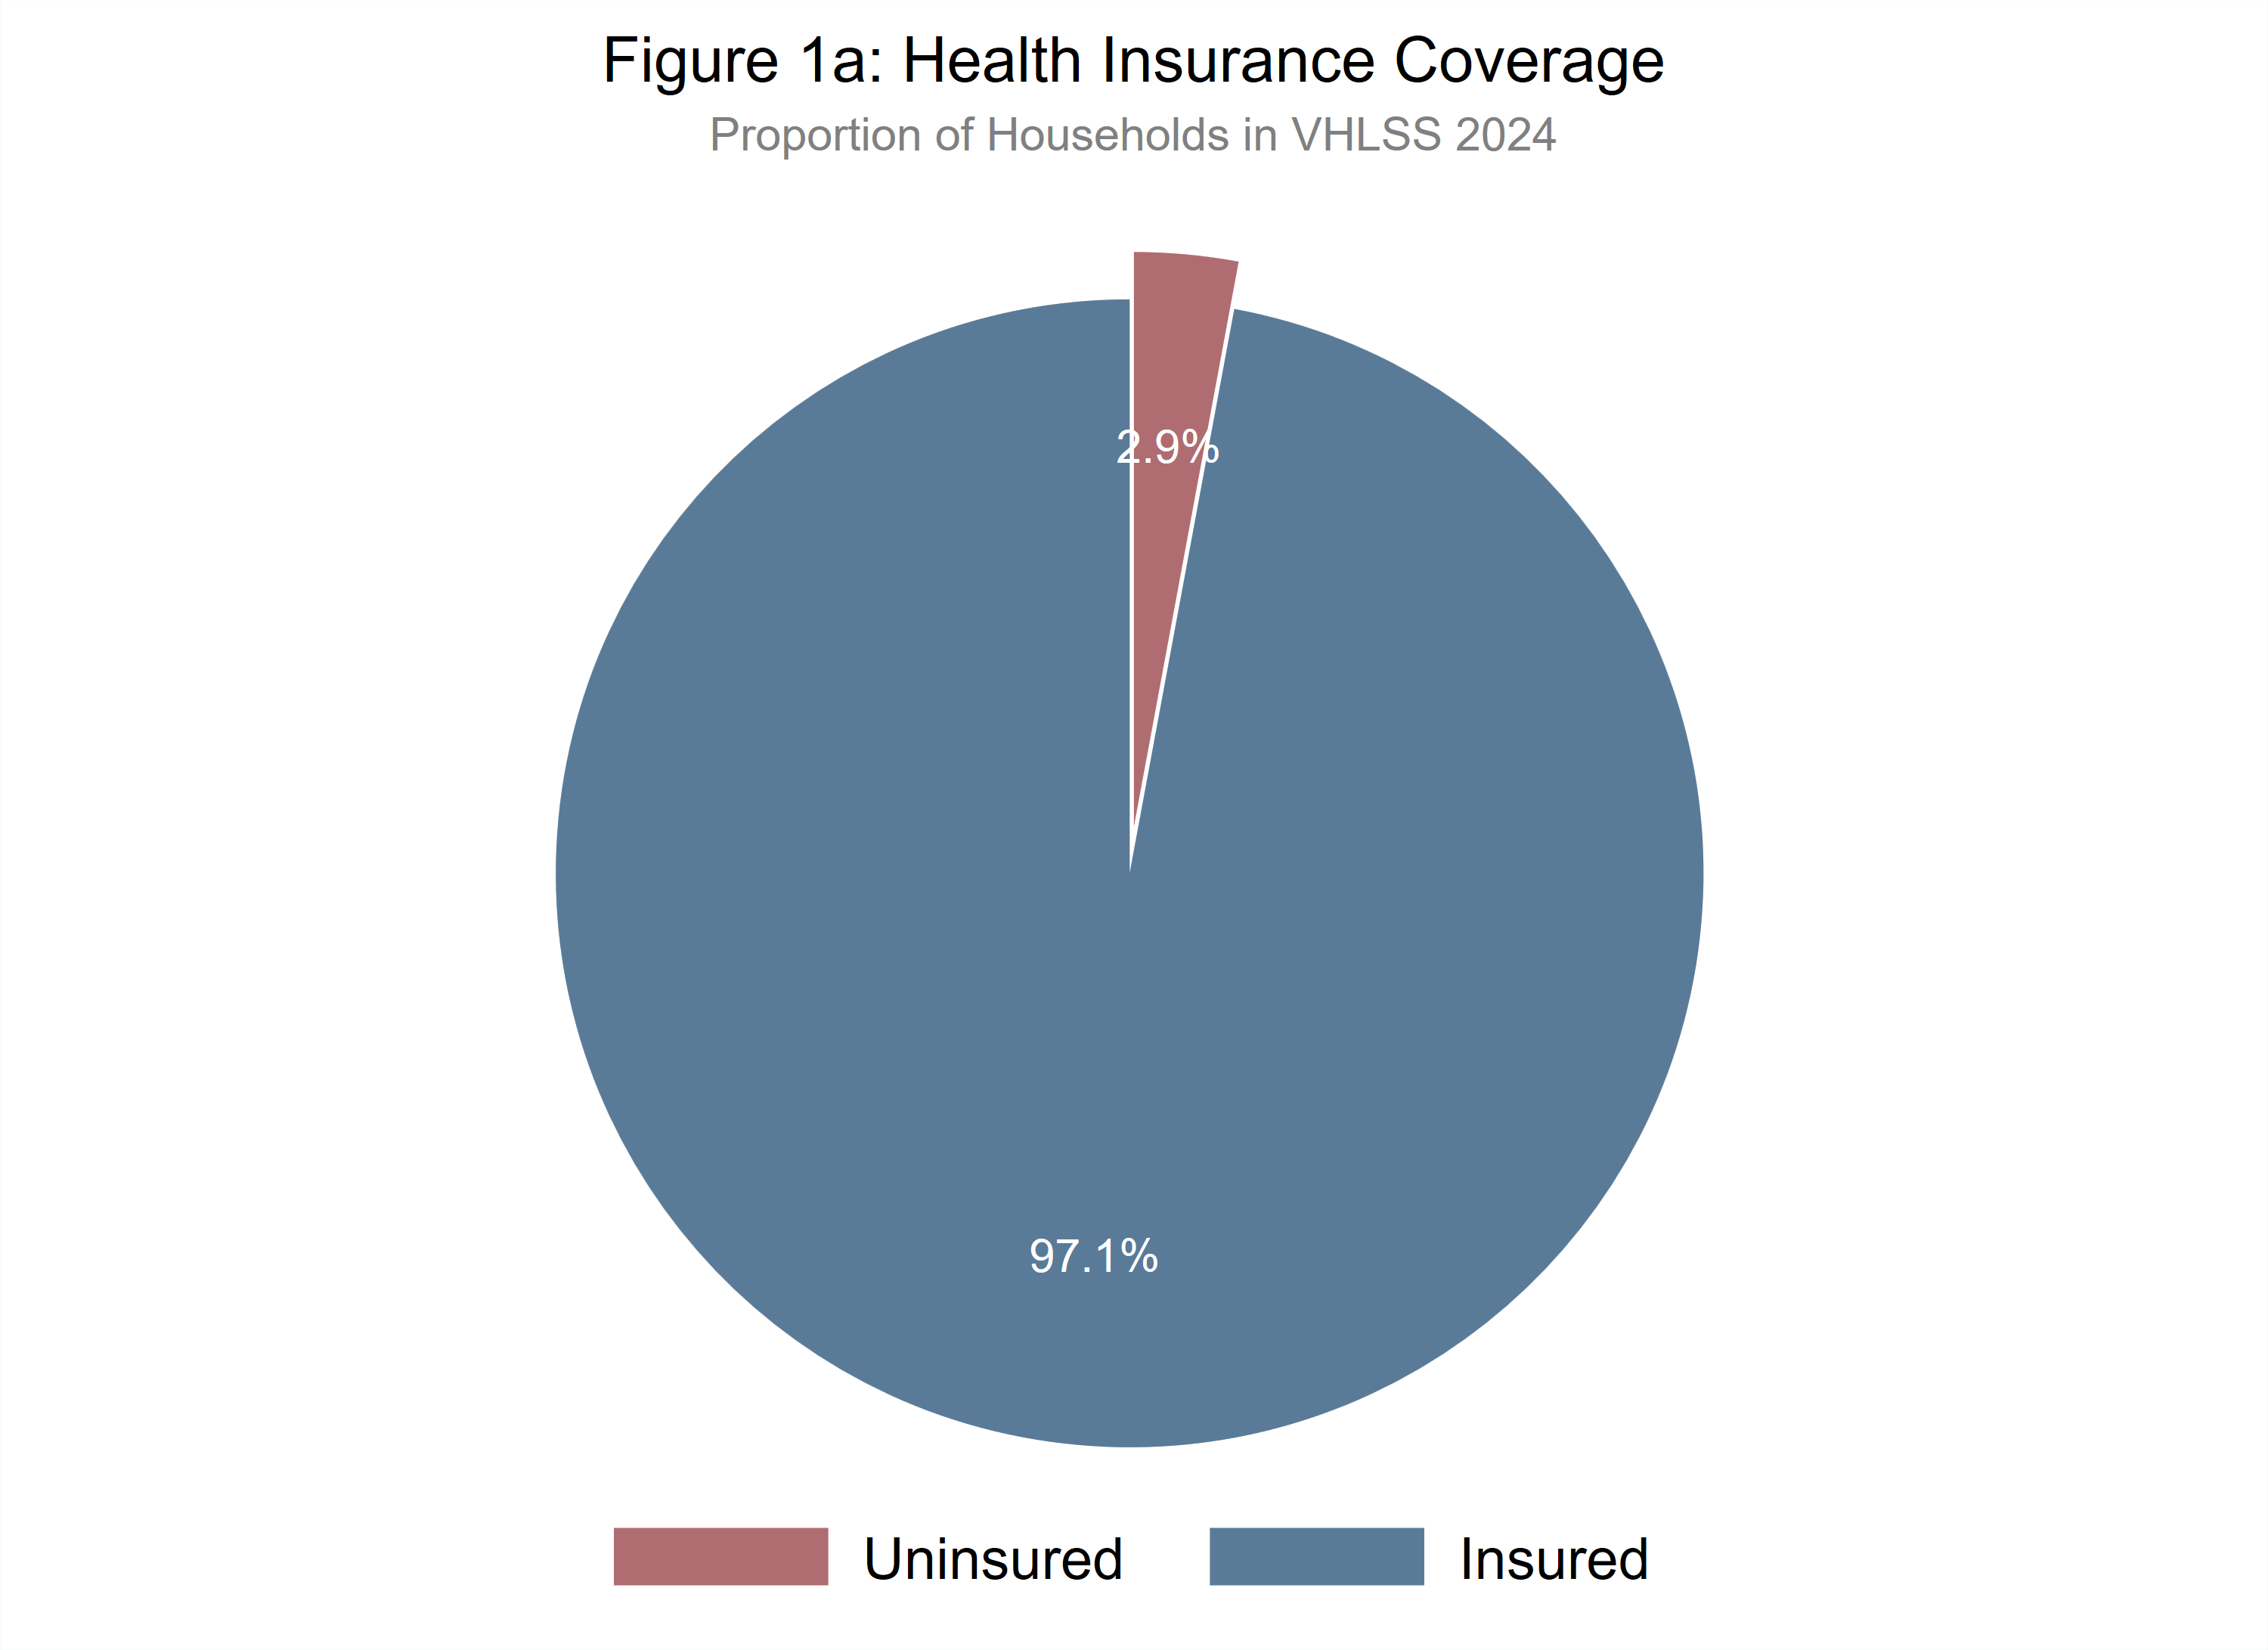
\includegraphics[width=0.75\textwidth]{Figure1a_Pie_BHYT.png}
	\caption{Tỷ lệ bao phủ Bảo hiểm Y tế của hộ gia đình (VHLSS 2024)}
	\label{fig:pie_bhyt}
\end{figure}

Khi bóc tách cấu trúc này, độ lệch chuẩn của chi phí nội trú ($10,278$) và giá trị tối đa cực đại ($600$ triệu VNĐ) cho thấy rủi ro tài chính thảm họa tập trung chủ yếu ở nhóm điều trị nội trú. Phần chênh lệch đáng kể còn lại phản ánh thói quen tự mua thuốc và sử dụng vật tư y tế ngoài danh mục. Đáng chú ý, có tới 37,5\% hộ gia đình ghi nhận hành vi tự ý khám chữa bệnh vượt tuyến, một yếu tố tiềm ẩn nguy cơ làm bùng nổ hình phạt đồng chi trả.

\begin{figure}[htbp]
	\centering
	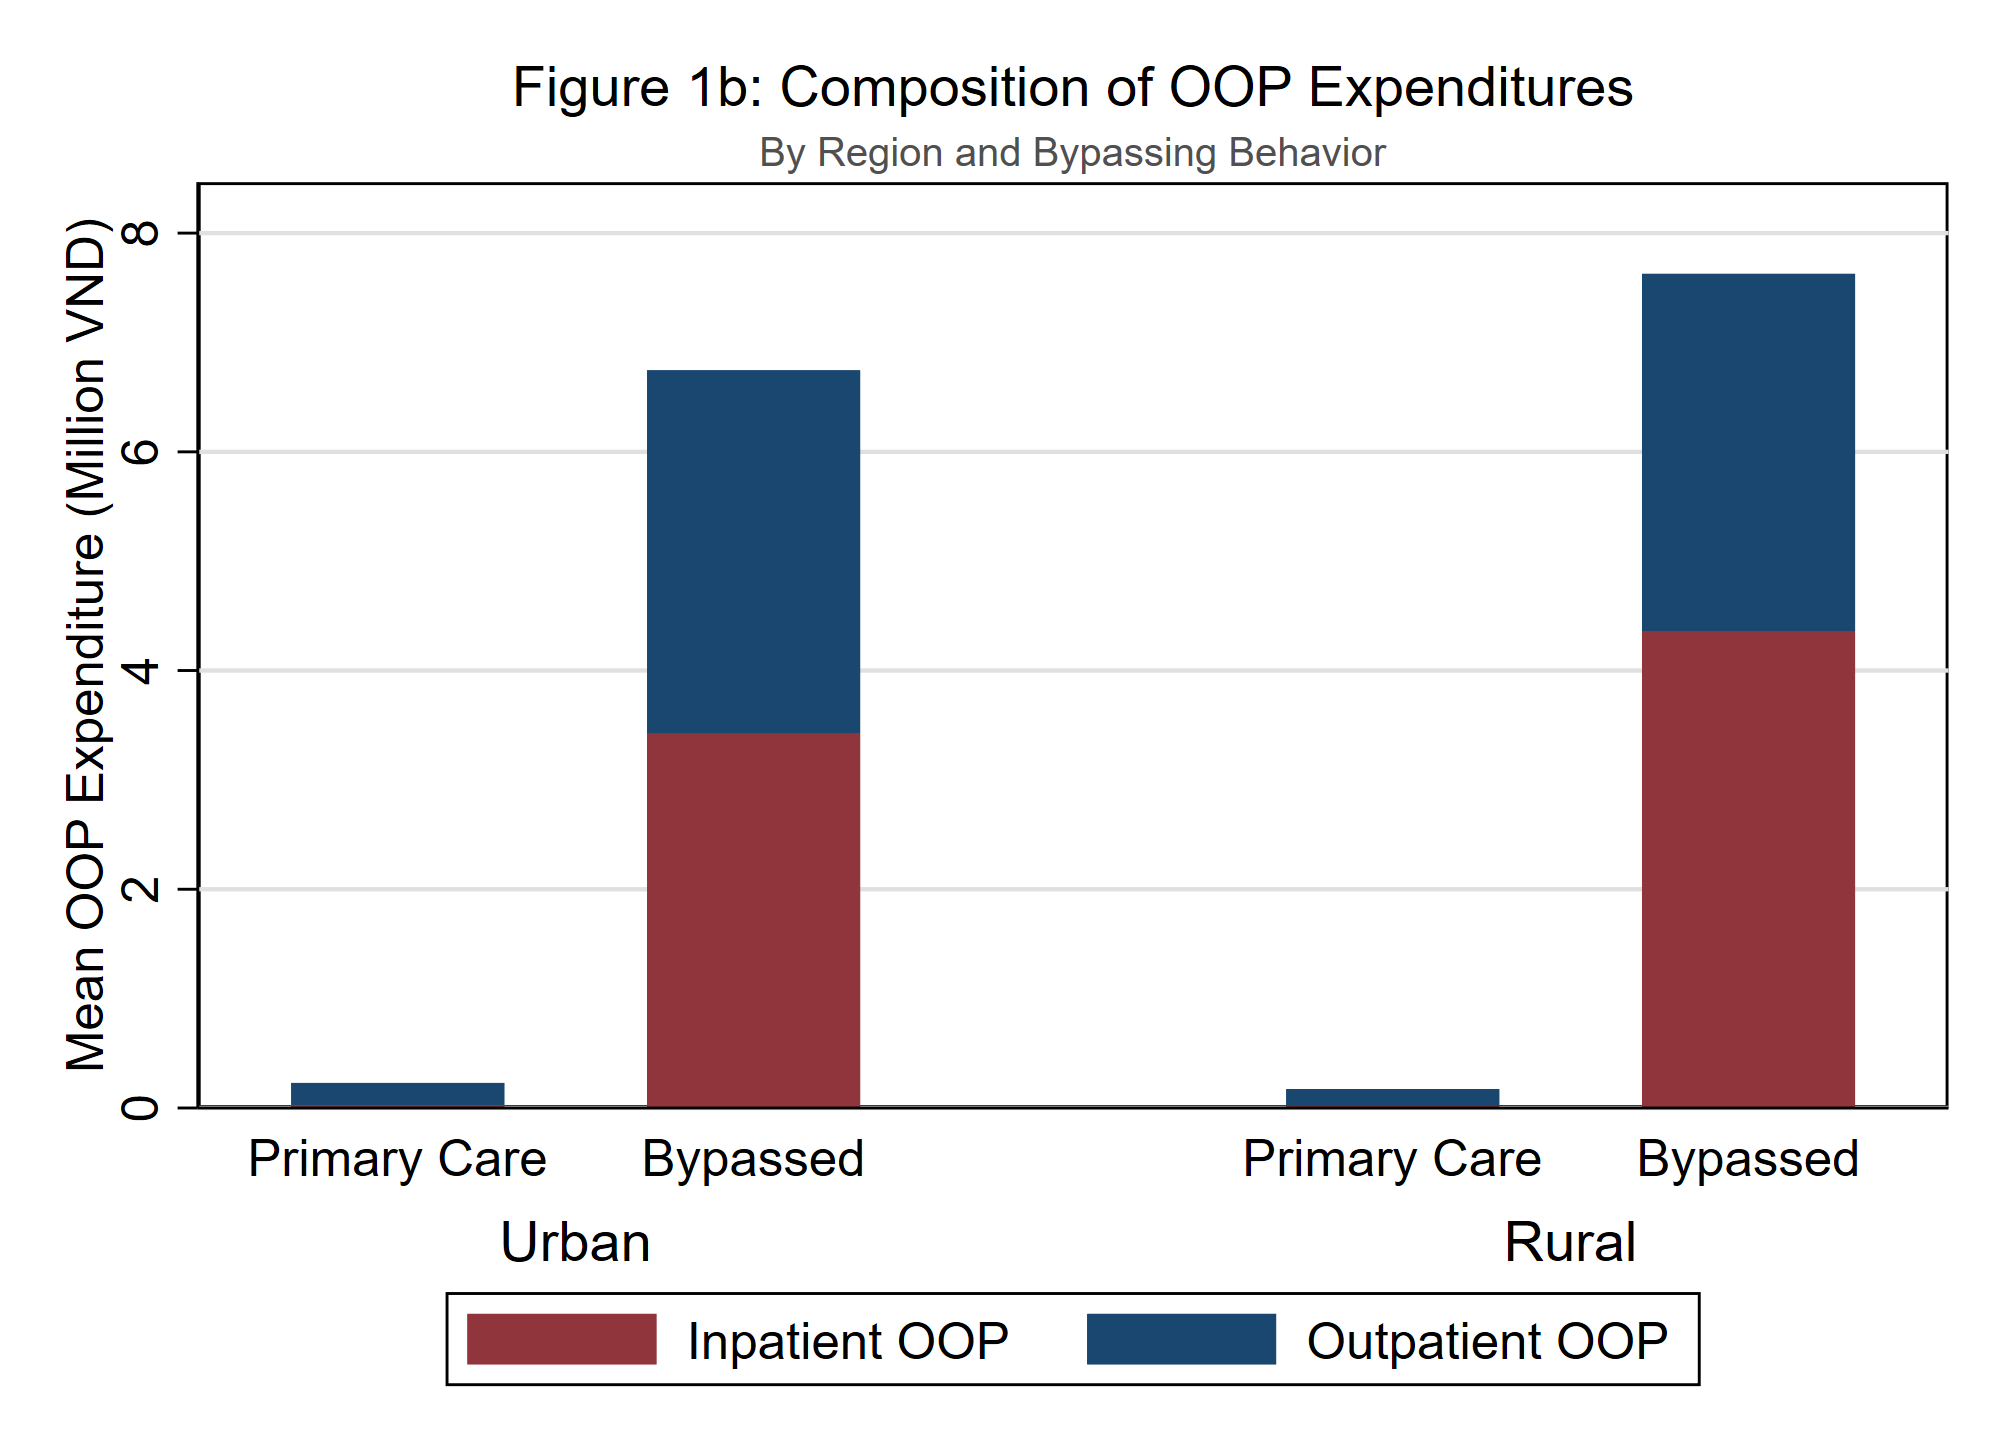
\includegraphics[width=0.85\textwidth]{figures/Figure1b_StackedBar_OOP.png}
	\caption{Cấu trúc chi phí y tế tiền túi phân theo Khu vực và Hành vi vượt tuyến}
	\label{fig:stacked_oop}
\end{figure}

Dữ liệu bộc lộ một thực tế bất đối xứng sắc nét (Hình \ref{fig:stacked_oop}): Tại khu vực nông thôn, nhóm vượt tuyến phải gánh chịu sự bùng nổ của chi phí OOP nội trú, hàm ý rằng họ thường chỉ chấp nhận chi phí tài chính rất cao để vượt tuyến khi đối mặt với các cú sốc sức khỏe nghiêm trọng. 

% --- ĐỒ THỊ BOXPLOT ---
\begin{figure}[htbp]
	\centering
	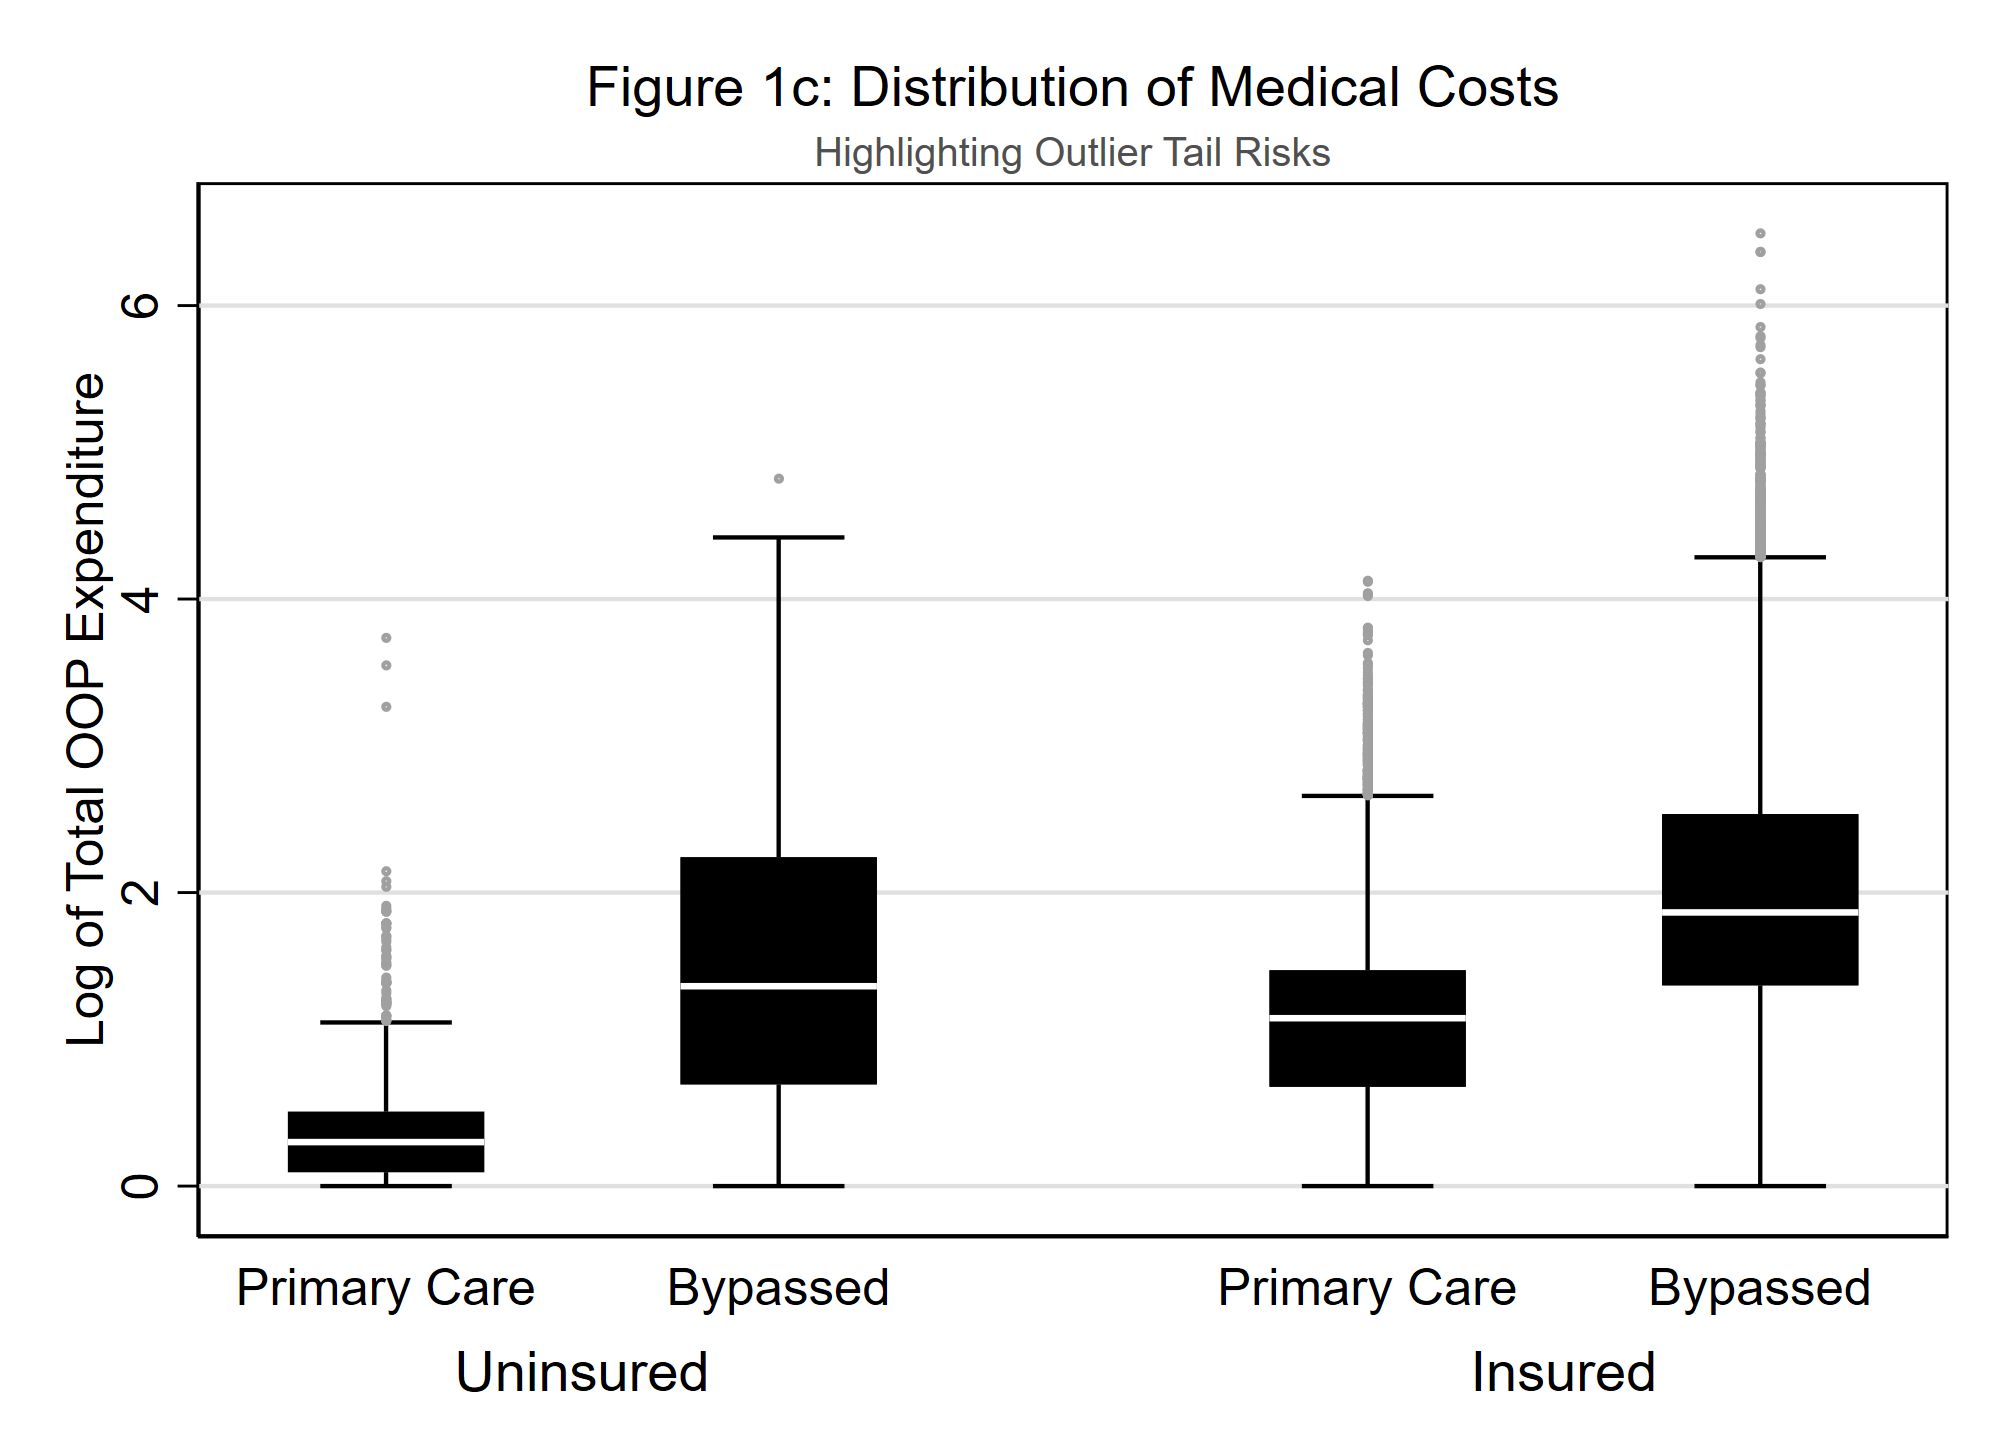
\includegraphics[width=0.85\textwidth]{figures/Figure1c_Boxplot_Bypass.png}
	\caption{Phân phối Log(OOP) nhấn mạnh rủi ro thảm họa y tế ở phần đuôi (Tail Risks)}
	\label{fig:boxplot_oop}
\end{figure}

Đặc điểm nổi bật nhất của chi phí OOP là sự phân phối lệch phải cực đoan. Việc sử dụng phép biến đổi logarit ($\ln\_OOP$) đã kéo phân phối về dạng tiệm cận chuẩn (Hình \ref{fig:kernel_density}). Đường mật độ của nhóm có BHYT dịch chuyển sang phải ở phần thân, hé lộ tín hiệu về hiệu ứng mở rộng: BHYT kích thích giải phóng nhu cầu y tế, đẩy tổng chi phí trung bình lên cao, nhưng lại giúp nén các cú sốc cực đoan ở phần đuôi phân phối.

% --- ĐỒ THỊ KERNEL DENSITY ---
\begin{figure}[htbp]
	\centering
	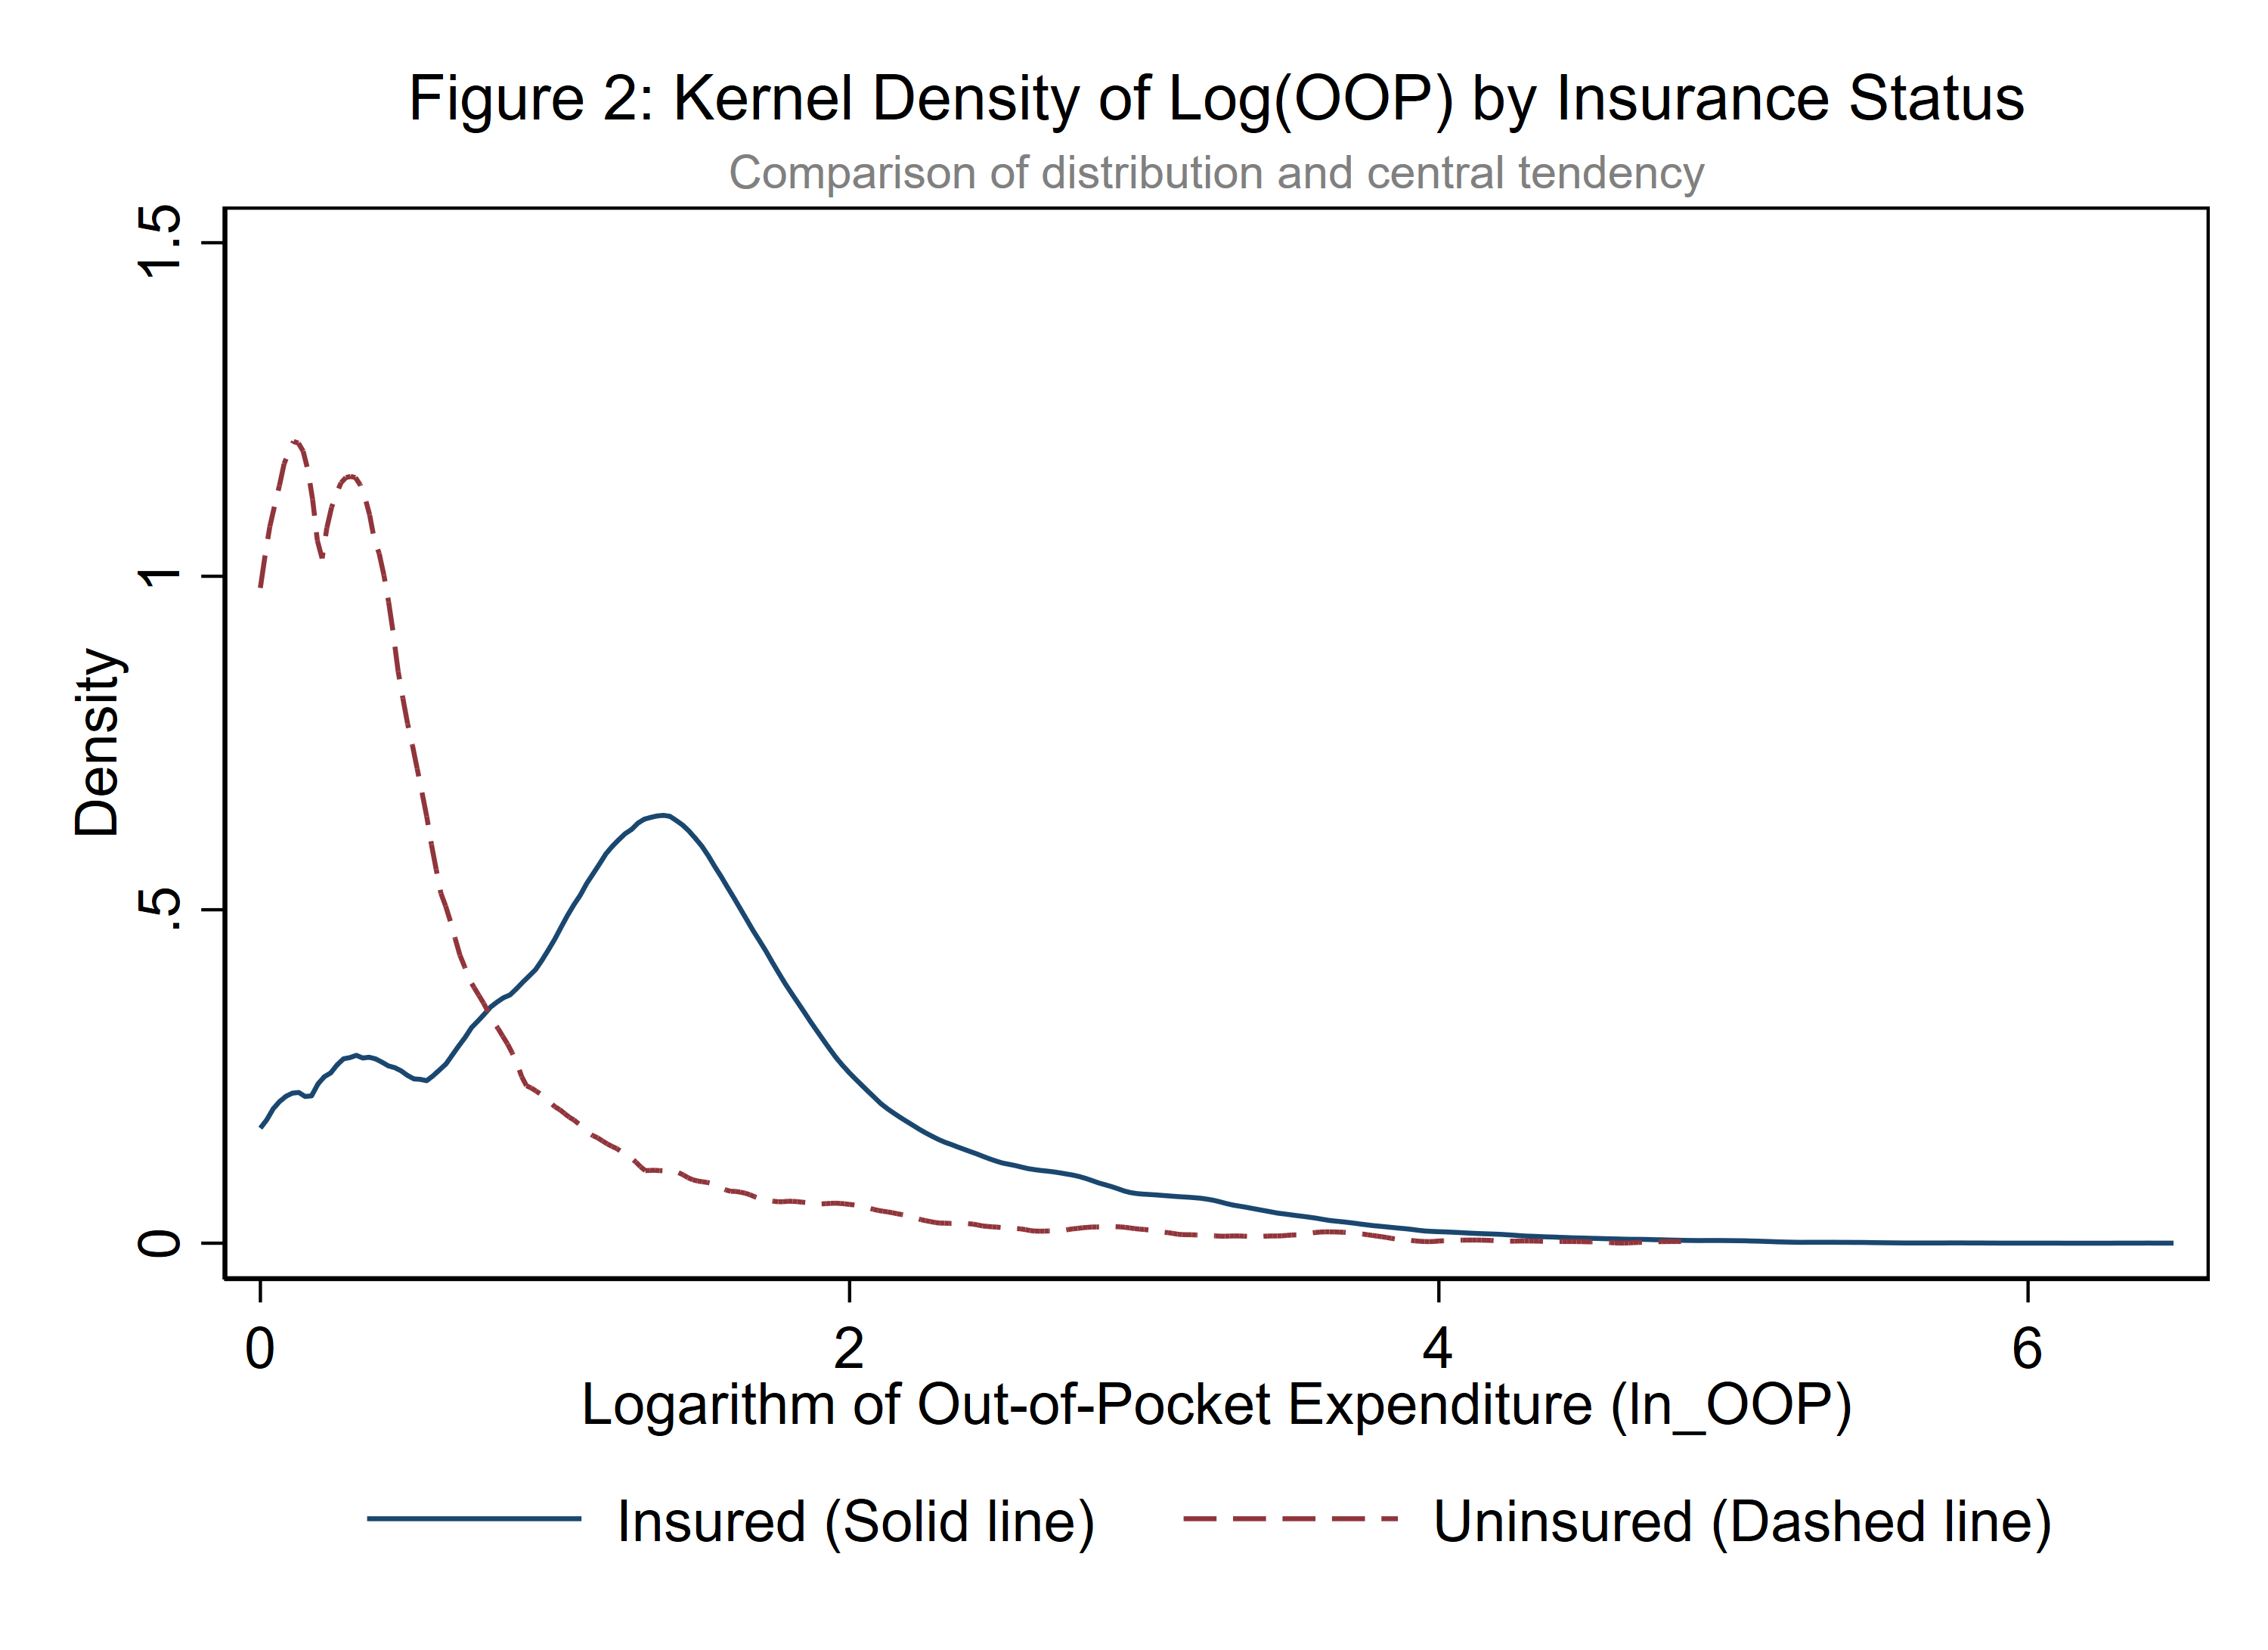
\includegraphics[width=0.8\textwidth]{figures/Figure2_Kernel_Density.png}
	\caption{Phân phối mật độ (Kernel Density) của Log chi tiêu y tế tiền túi theo trạng thái BHYT}
	\label{fig:kernel_density}
\end{figure}

\clearpage
\subsection{Hiệu ứng kép của BHYT}

Kết quả từ mô hình IV-2SLS (Bảng \ref{tab:decomposed_oop}) cung cấp bằng chứng thực nghiệm mạnh mẽ về sự tồn tại của Hiệu ứng kép có tính chất phi tuyến trong cơ chế vận hành của BHYT.

\begin{table}[htbp]
	\centering
	\def\sym#1{\ifmmode^{#1}\else\(^{#1}\)\fi}
	\caption{Tác động của BHYT lên cấu trúc chi phí OOP phân rã (Mô hình IV-2SLS)}
	\label{tab:decomposed_oop}
	\begin{tabular}{lccc}
		\toprule
		&\textbf{(1)}&\textbf{(2)}&\textbf{(3)}\\
		\textbf{Biến độc lập}&\textbf{Log(Tổng OOP)}&\textbf{Log(OOP Nội trú)}&\textbf{Log(OOP Ngoại trú)}\\
		\midrule
		BHYT (Cơ sở) & 1.256\sym{***} & -0.219 & 0.292\sym{*} \\
		& (0.177) & (0.155) & (0.157) \\
		\addlinespace
		BHYT $\times$ Nông thôn & -0.967\sym{***} & -0.115 & 0.035 \\
		& (0.286) & (0.178) & (0.137) \\
		\addlinespace
		BHYT $\times$ Vượt tuyến & 2.413 & 2.806 & 0.405 \\
		& (1.833) & (2.172) & (1.513) \\
		\addlinespace
		BHYT $\times$ Nông thôn $\times$ Vượt tuyến & -3.533 & -1.345 & -2.971\sym{*} \\
		& (2.151) & (2.431) & (1.707) \\
		\addlinespace
		Nông thôn (Base) & 0.850\sym{***} & 0.083 & -0.026 \\
		& (0.262) & (0.155) & (0.133) \\
		\addlinespace
		Vượt tuyến (Base) & -1.648 & -2.244 & 0.443 \\
		& (1.795) & (2.092) & (1.493) \\
		\midrule
		Biến kiểm soát ($X$) & Có & Có & Có \\
		Fixed Effects (Tỉnh) & Có & Có & Có \\
		\midrule
		Số quan sát ($N$) & 46.995 & 46.995 & 46.995 \\
		\bottomrule
		\multicolumn{4}{p{13cm}}{\footnotesize \textit{Ghi chú:} Sai số chuẩn vững (Robust standard errors) được cụm theo cấp tỉnh đặt trong ngoặc đơn. \newline \sym{*} \(p<0.10\), \sym{**} \(p<0.05\), \sym{***} \(p<0.01\)}
	\end{tabular}
\end{table}

 Hệ số $+1.256$ của biến BHYT cơ sở trong mô hình Log-Linear ngụ ý rằng, trung bình, việc sở hữu thẻ BHYT làm gia tăng chi phí OOP tổng thể lên khoảng $251\%$. Căn cứ trên mức chi tiêu OOP trung bình của mẫu là $5.578$ triệu VNĐ/hộ/năm, sự gia tăng này tương đương với khoảng $14$ triệu VNĐ. Mặc dù con số này thoạt nhìn khá cao, nhưng nó hoàn toàn logic với hiện trạng cấu trúc y tế Việt Nam hiện nay, nơi hiện tượng cầu do nhà cung cấp tạo ra kết hợp với rủi ro đạo đức, khiến tỷ trọng thuốc ngoài danh mục và dịch vụ kỹ thuật cao tự nguyện bị đẩy lên mức đỉnh điểm. Kết quả này cũng tiệm cận với các ước lượng trước đây của \textcite{wagstaff2007} và đồng nhất với các cảnh báo của Bộ Y tế về đà tăng trưởng nóng của chi phí y tế hộ gia đình trong giai đoạn hậu đại dịch.

% --- ĐỒ THỊ FOREST PLOT (HIỆU ỨNG KÉP) ---
\begin{figure}[htbp]
	\centering
	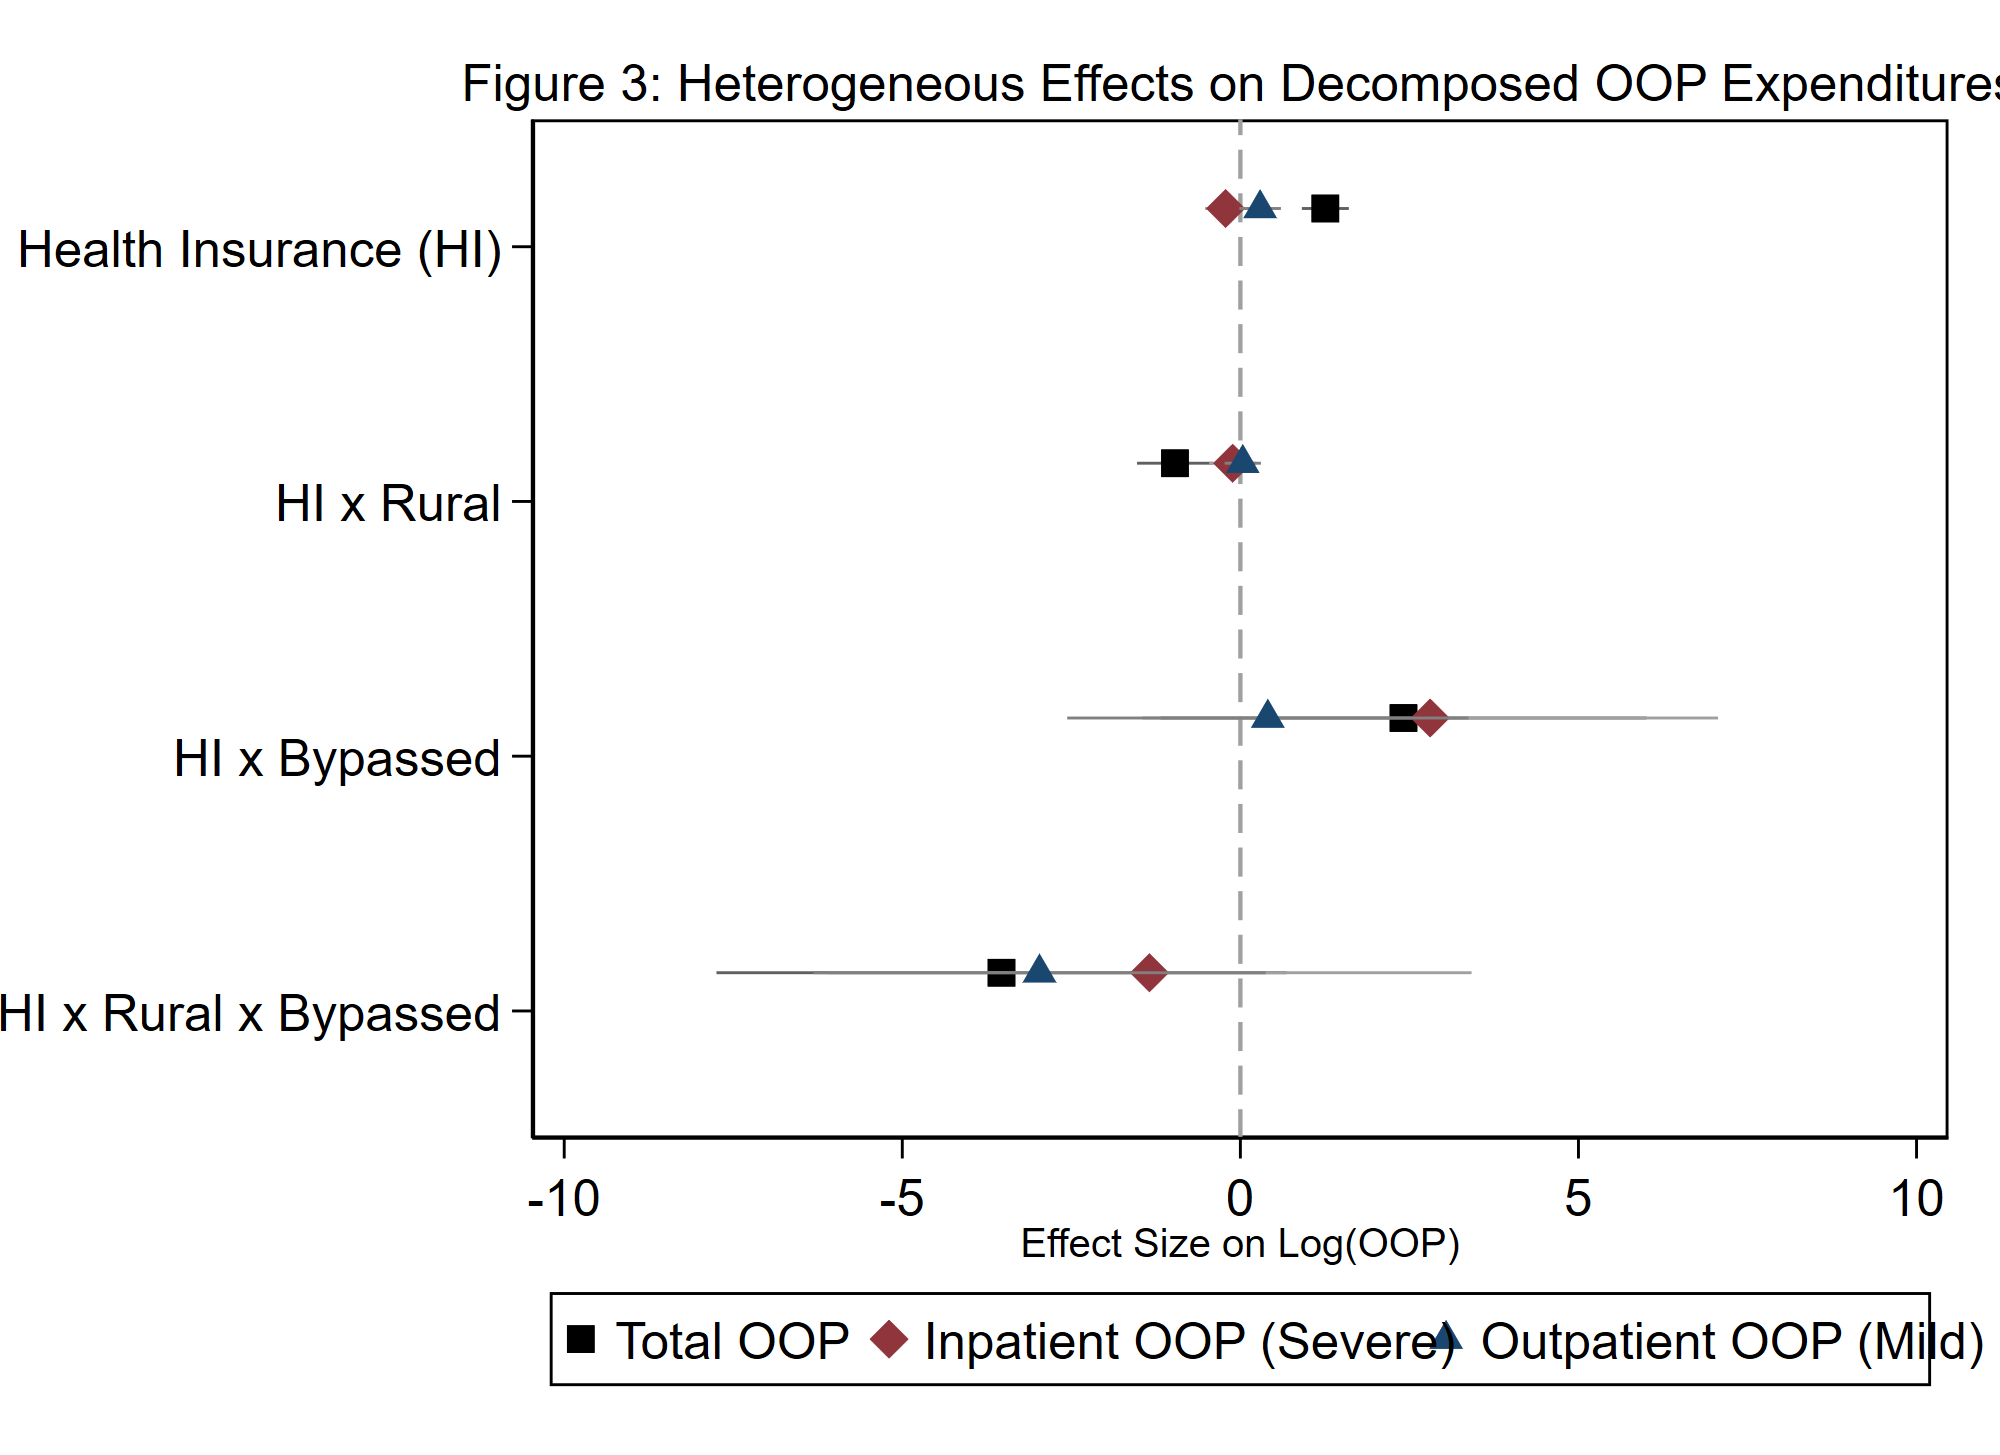
\includegraphics[width=0.9\textwidth]{figures/Figure3_Combined_ForestPlot.png}
	\caption{Hiệu ứng phân hóa của BHYT lên cấu trúc chi phí OOP (Combined Forest Plot)}
	\label{fig:forest_plot}
\end{figure}

Sự đối lập trong cơ chế tác động của BHYT được biểu diễn trực quan thông qua Forest Plot (Hình \ref{fig:forest_plot}), phơi bày hai mảng sáng và tố của chính sách BHYT:

\begin{itemize}
	\item \textbf{Kích thích tiếp cận ở Ngoại trú (Hiệu ứng mở rộng):} Ở Cột (3), hệ số BHYT cơ sở mang dấu dương ($+0.292, p < 0.10$). Điều này xác nhận rằng với các dịch vụ nhẹ, việc sở hữu thẻ BHYT đã gỡ bỏ rào cản tài chính ban đầu, khai thông lượng nhu cầu y tế vốn bị kìm nén trước đây. Sự gia tăng tần suất sử dụng dịch vụ kéo theo sự phình to của các khoản đồng chi trả và chi phí tự mua thuốc bên ngoài, làm tăng mức OOP ngoại trú nói chung.
	
	\item \textbf{Lưới an sinh tại nông thôn và tác động răn đe khi vượt tuyến:} Trái ngược với hiệu ứng tăng chi phí ở nhóm cơ sở, BHYT thể hiện sức mạnh bảo vệ tài chính rõ rệt đối với các nhóm yếu thế. Tại Cột (1), tương tác 2 chiều ($BHYT \times N\hat{o}ng\ th\hat{o}n$) tạo ra lực cản giảm Tổng OOP rất mạnh ($-0.967, p < 0.01$). Đặc biệt hơn, tại Cột (3), biến tương tác 3 chiều ($BHYT \times N\hat{o}ng\ th\hat{o}n \times V\mathopen{ư}\mathclose{ợ}t\ tuy\acute{ế}n$) ghi nhận mức giảm kỷ lục ($-2.971, p < 0.10$). Các cơ chế hình phạt tài chính của BHYT đối với hành vi vượt tuyến đang hoạt động cực kỳ hiệu quả ở nhóm bệnh nhân nông thôn trong các ca ngoại trú, giúp định tuyến bệnh nhân và ngăn chặn tình trạng đổ xô lên tuyến trên không cần thiết.
	
	\item \textbf{Khoảng trống trong bảo vệ nội trú:} Đáng chú ý, toàn bộ các hệ số tại Cột (2) (OOP Nội trú) đều không đạt mức ý nghĩa thống kê. Sự thiếu vắng này phản ánh một thực tế lâm sàng: chi phí điều trị nội trú có độ phân tán vô cùng cực đoan. Khi hóa đơn viện phí vượt quá trần thanh toán, thẻ bảo hiểm chưa thể hiện được sự khác biệt tuyến tính trên mức trung bình mẫu, đòi hỏi các phân tích chuyên sâu hơn ở phần đuôi của phân phối chi phí.
\end{itemize}

\clearpage
\subsection{Tác động dọc theo phân phối thảm họa (SQREG)}

Để đánh giá sự thay đổi trong cơ chế bảo vệ của BHYT khi đối mặt với các cú sốc y tế lớn, nghiên cứu sử dụng mô hình Hồi quy phân vị đồng thời (SQREG). 

\begin{table}[htbp]
	\centering
	\def\sym#1{\ifmmode^{#1}\else\(^{#1}\)\fi}
	\caption{Tóm tắt tác động của BHYT và hành vi Vượt tuyến theo phân vị chi phí}
	\label{tab:sqreg_summary}
	\begin{tabular}{lcccc}
		\toprule
		&\textbf{(1)}&\textbf{(2)}&\textbf{(3)}&\textbf{(4)}\\
		\textbf{Biến độc lập}&\textbf{Q25}&\textbf{Q50}&\textbf{Q75}&\textbf{Q90}\\
		\midrule
		Vượt tuyến & 0.558\sym{***} & 0.916\sym{***} & 1.654\sym{***} & 2.039\sym{***} \\
		& (0.081) & (0.088) & (0.121) & (0.228) \\
		\addlinespace
		BHYT $\times$ Vượt tuyến & -0.045 & -0.290\sym{***} & -0.643\sym{***} & -0.605\sym{***} \\
		& (0.083) & (0.090) & (0.125) & (0.228) \\
		\midrule
		Các biến kiểm soát & Có & Có & Có & Có \\
		\midrule
		Pseudo $R^2$ & 0.202 & 0.209 & 0.260 & 0.314 \\
		Số quan sát ($N$) & \multicolumn{4}{c}{46.995} \\
		\bottomrule
		\multicolumn{5}{p{13cm}}{\footnotesize \textit{Ghi chú:} Bảng chỉ hiển thị các hệ số trọng tâm. Sai số chuẩn bootstrap (100 lần lặp) trong ngoặc đơn. \sym{***} \(p<0.01\)}
	\end{tabular}
\end{table}

Kết quả SQREG xác nhận sự leo thang tuyến tính của hình phạt vượt tuyến dọc theo phân phối chi phí. Hệ số của hành vi vượt tuyến tăng phi mã từ $0.558$ ở nhóm chi tiêu thấp ($Q25$) lên đến mức thảm họa $2.039$ ở đỉnh rủi ro ($Q90$). 

Đáng chú ý, chính tại phân vị cực đoan $Q90$ này, thẻ BHYT mới phát huy uy lực bảo vệ lớn nhất. Hệ số tương tác ($BHYT \times Vượt tuyến$) chuyển từ trạng thái không có ý nghĩa thống kê ở $Q25$ sang mức cản phá mạnh mẽ $-0.605$ ($p < 0.01$) tại $Q90$. Dù BHYT không ngăn được hoàn toàn chi phí dội lên do tự ý vượt tuyến, nó đóng vai trò như một chiếc phanh hãm khẩn cấp, giúp bệnh nhân khỏi nguy cơ phá sản y tế khi hóa đơn chạm ngưỡng thảm họa.

\clearpage
\subsection{Nhận diện nguyên nhân thể chế: So sánh với Thái Lan thông qua TVSEP}

Từ kết quả phân tích trên ta có thể đặt câu hỏi: Tại sao BHYT lại tạo ra Hiệu ứng mở rộng mạnh nhưng vẫn để bỏ sót nhiều ca thảm họa tại Việt Nam? Để trả lờitục câu hỏi trên, nghiên cứu tiếp tục đối chiếu cấu trúc thể chế với Thái Lan thông qua dữ liệu mảng TVSEP (2007-2024).

% --- ĐỒ THỊ XU HƯỚNG TỔNG QUAN TVSEP ---
\begin{figure}[htbp]
	\centering
	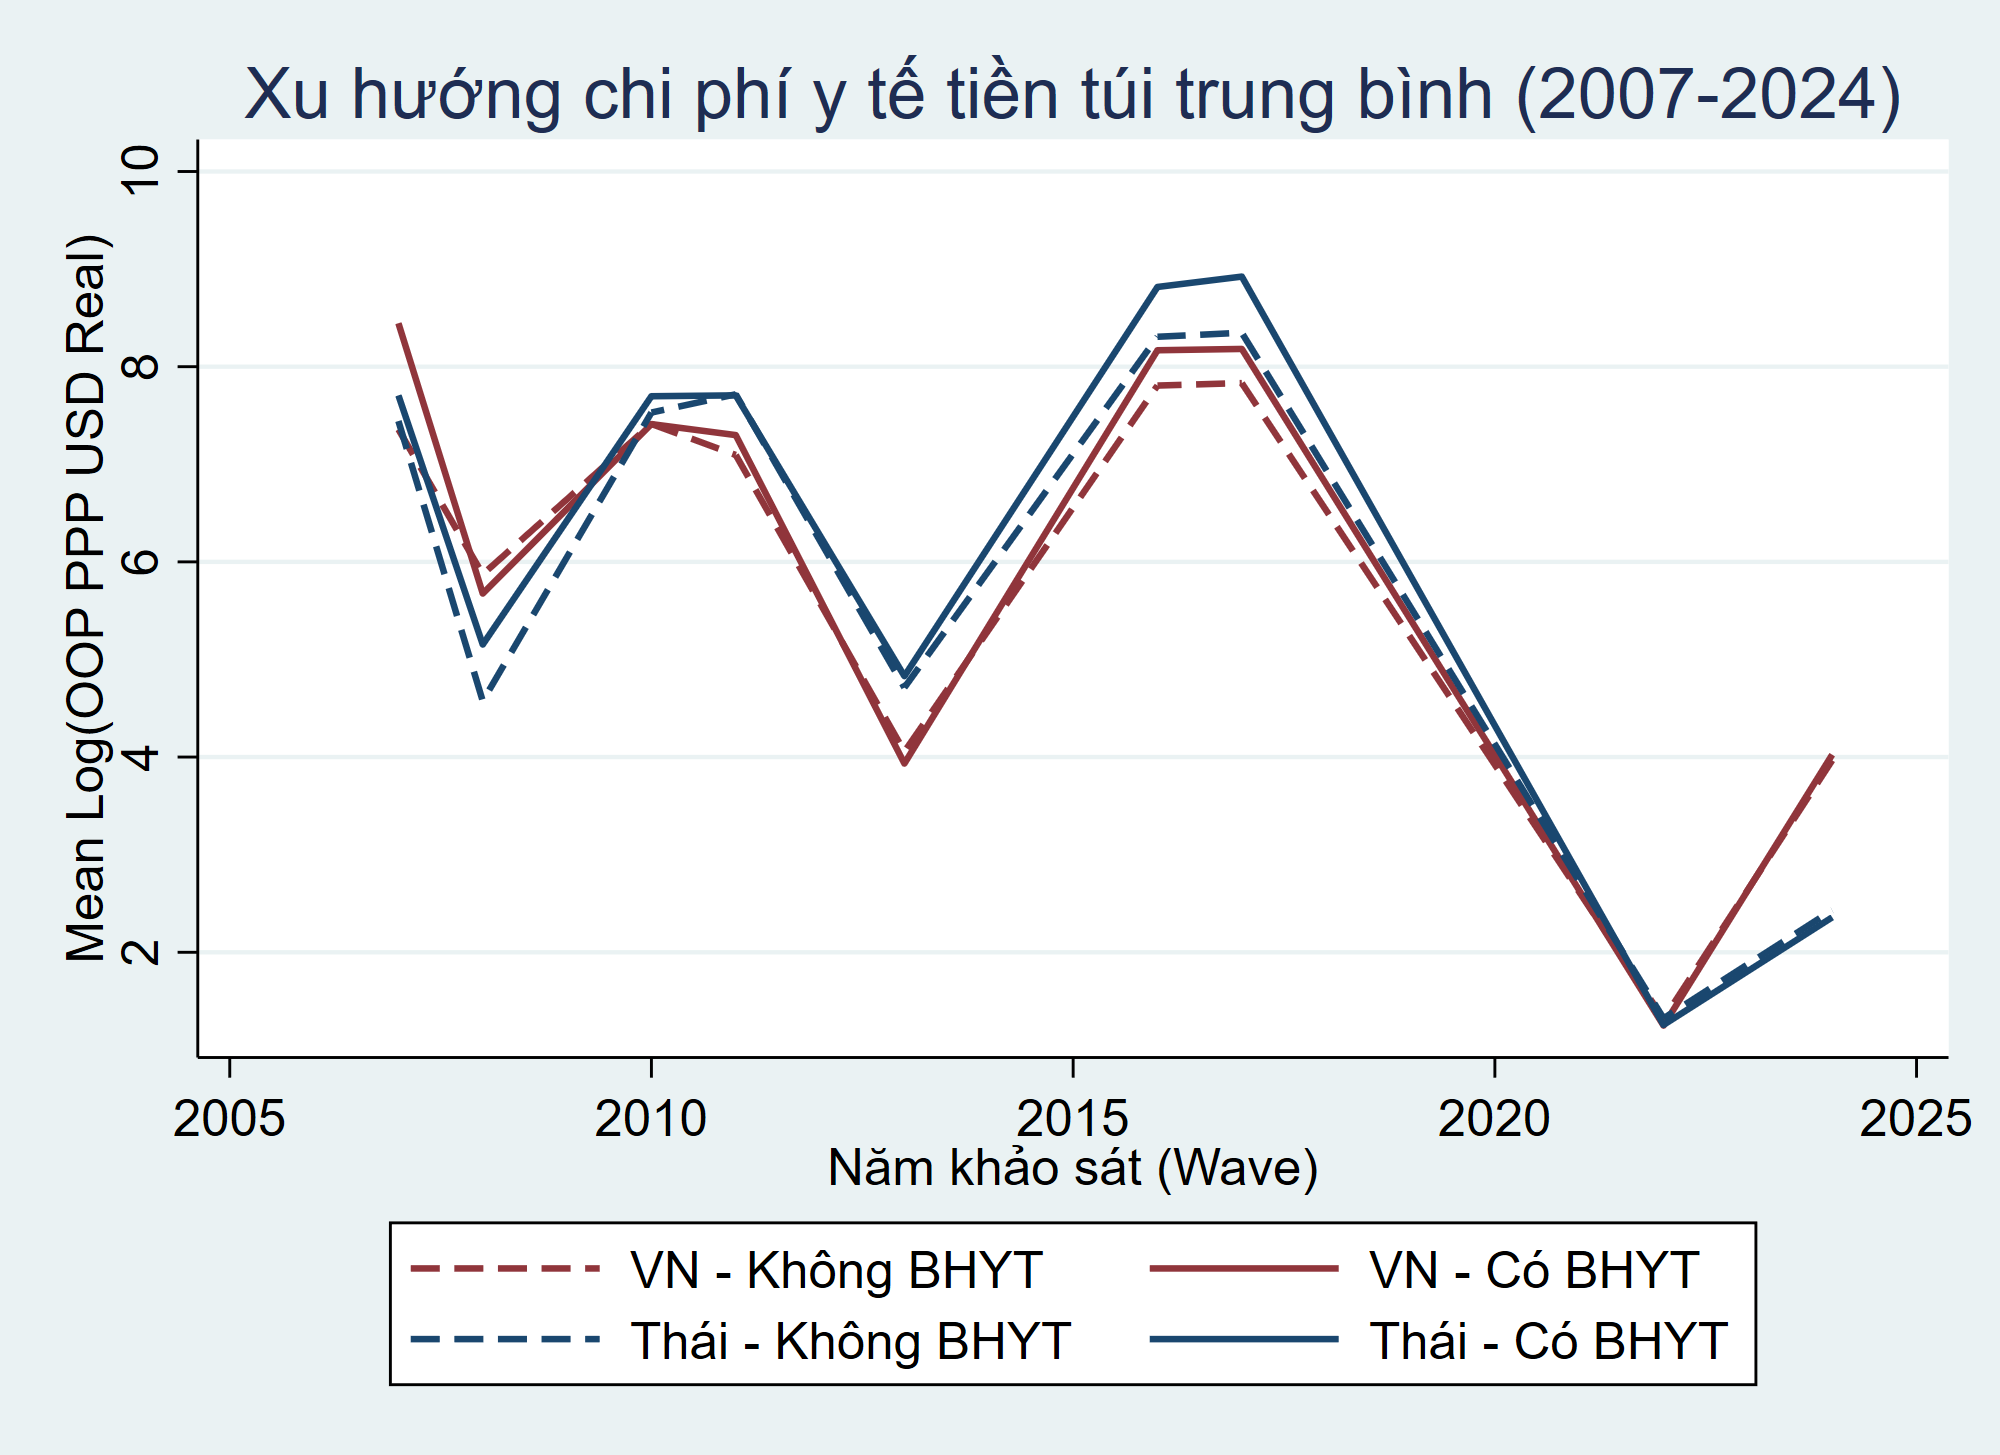
\includegraphics[width=0.9\textwidth]{figures/oop_trend_overall.png}
	\caption{Xu hướng chi phí y tế tiền túi trung bình tại Việt Nam và Thái Lan (2007-2024)}
	\label{fig:tvsep_trend}
\end{figure}

Xu hướng chi phí y tế tiền túi có sự phân kỳ rõ rệt giữa hai quốc gia (Hình \ref{fig:tvsep_trend}). BHYT ở Việt Nam đi kèm với mức chi tiêu OOP dao động mạnh và có xu hướng tăng, trong khi đó quỹ đạo này ở Thái Lan tỏ ra bằng phẳng và được kiểm soát tốt hơn nhiều.

\begin{table}[htbp]
	\centering
	\def\sym#1{\ifmmode^{#1}\else\(^{#1}\)\fi}
	\caption{Tác động chênh lệch thể chế đến OOP (Việt Nam so với Thái Lan)}
	\label{tab:tvsep_results}
	\begin{tabular}{lcc}
		\toprule
		\textbf{Biến độc lập}&\textbf{Baseline (TWFE Mean)}&\textbf{Catastrophic (Q90)}\\
		\midrule
		BHYT (Chung - VN) & -0.077 & 0.301\sym{***} \\
		BHYT $\times$ Thái Lan & 0.554\sym{***} & -0.690\sym{***} \\
		Vượt tuyến (Chung - VN) & 0.065\sym{***} & -0.354\sym{***} \\
		Vượt tuyến $\times$ Thái Lan & 0.014 & 0.395\sym{***} \\
		\midrule
		Kiểm soát FE Hộ \& Năm & Có & Có \\
		Số quan sát ($N$) & 23.754 & 29.473 \\
		\bottomrule
		\multicolumn{3}{p{10cm}}{\footnotesize \textit{Ghi chú:} Phụ thuộc: Log(OOP PPP USD Real). \sym{***} \(p<0.01\)}
	\end{tabular}
\end{table}

Kết quả mô hình TVSEP (Bảng \ref{tab:tvsep_results}) bộc lộ sự tương phản hệ thống như sau:
\begin{itemize}
	\item Tại ngưỡng trung bình, tương tác $BHYT \times Th\acute{a}i\ Lan$ có hệ số dương ($0.554$), chứng tỏ cơ chế Bao phủ toàn dân (UCS) của Thái Lan khơi thông tiếp cận y tế cơ bản tốt hơn.
	
	\item Tuy nhiên, tại ngưỡng thảm họa (Q90), cơ chế Khoán định suất kết hợp Người gác cổng của Thái Lan thể hiện sức mạnh tuyệt đối. Biến tương tác mang dấu âm lớn ($-0.690, p < 0.01$), chặn đứng rủi ro thảm họa hiệu quả hơn hẳn so với cơ chế Phí dịch vụ của Việt Nam , nơi các bệnh viện tuyến trên có động cơ tối đa hóa doanh thu từ bệnh nhân nặng.
\end{itemize}

% --- ĐỒ THỊ BOXPLOT SO SÁNH PHÂN PHỐI ---
\begin{figure}[htbp]
	\centering
	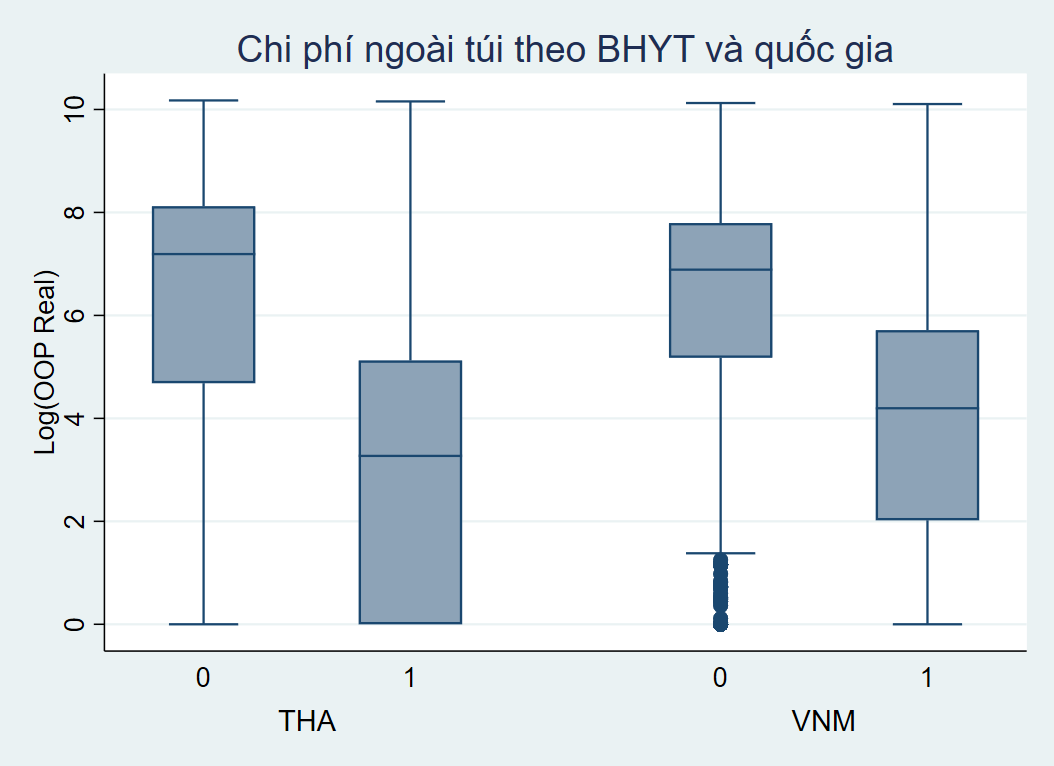
\includegraphics[width=0.85\textwidth]{figures/gbox_ins_country.png}
	\caption{Phân phối chi phí y tế tiền túi (Log OOP) theo trạng thái BHYT và Quốc gia}
	\label{fig:tvsep_boxplot}
\end{figure}

Phân phối chi phí (Hình~\ref{fig:tvsep_boxplot}) cùng với phân tích động học theo thời gian bằng phương pháp \textit{event-study} (Hình~\ref{fig:tvsep_dynamic}) cung cấp bằng chứng thực nghiệm quan trọng về sự phân kỳ trong quỹ đạo chi phí giữa hai hệ thống y tế. Kết quả cho thấy tác động biên của BHYT tại Việt Nam (đường màu đỏ) có xu hướng gia tăng rõ rệt sau các đợt cải cách hệ thống y tế năm 2014 và đặc biệt là sau khi triển khai chính sách thông tuyến năm 2016. Trong khi đó, quỹ đạo của Thái Lan tương đối ổn định trong suốt giai đoạn quan sát kéo dài 17 năm.

% --- ĐỒ THỊ DYNAMIC EFFECT (EVENT-STUDY) ---
\begin{figure}[htbp]
	\centering
	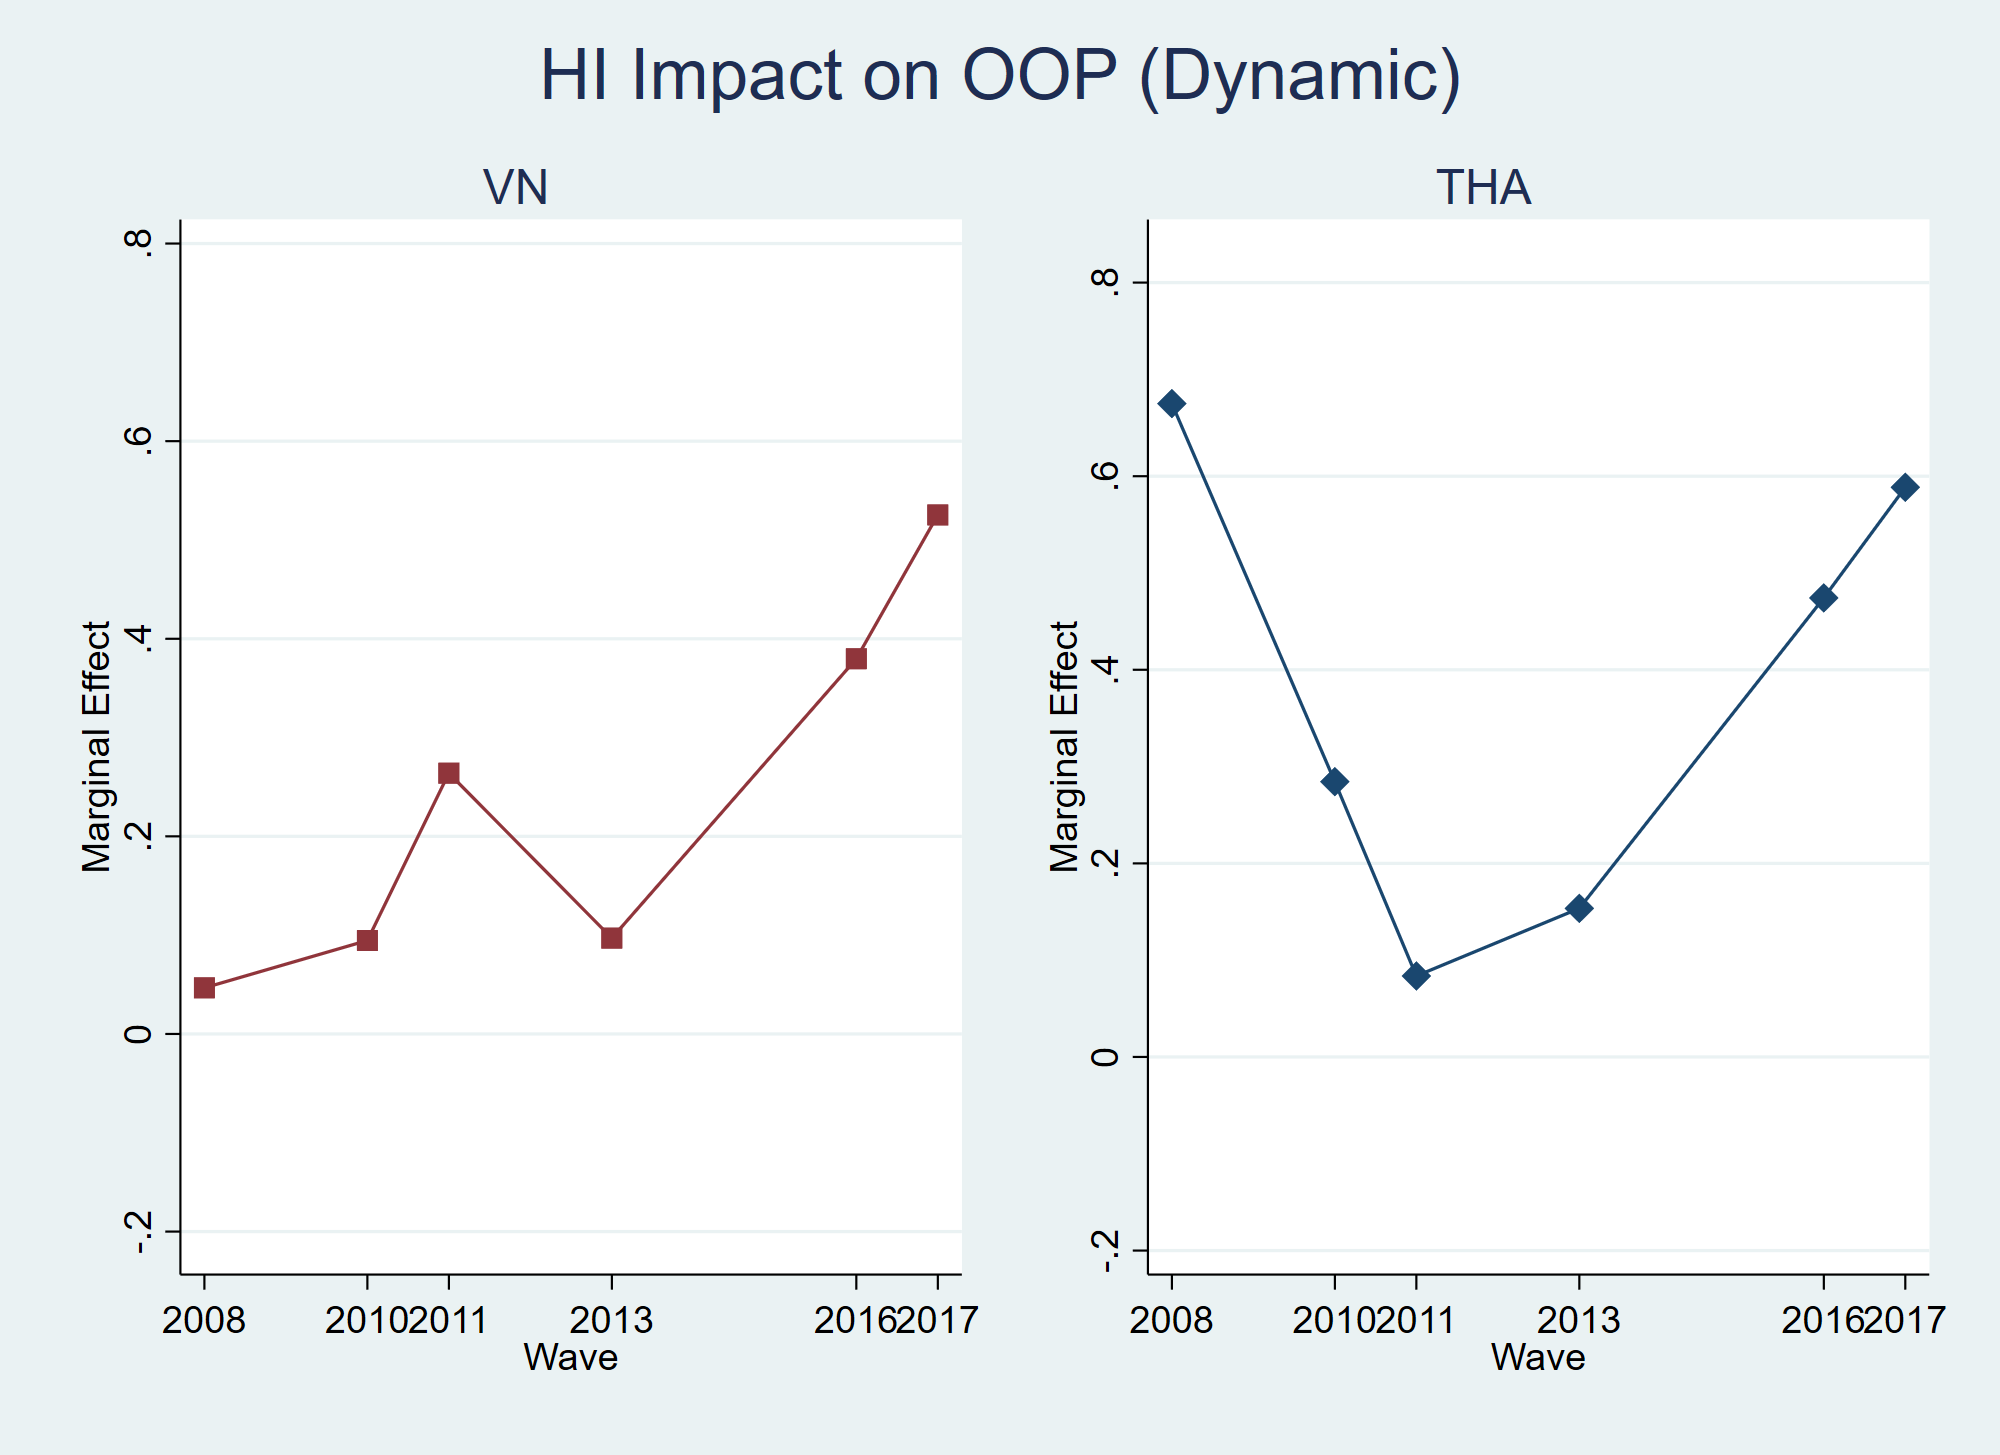
\includegraphics[width=1\textwidth]{figures/g_dynamic_effect.png}
	\caption{Dynamic Effects của BHYT lên OOP qua các năm của Việt Nam so với Thái Lan}
	\label{fig:tvsep_dynamic}
\end{figure}

Sự khác biệt này có thể được lý giải từ góc độ thiết kế thể chế của hệ thống y tế. Tại Thái Lan, mạng lưới an sinh y tế được xây dựng dựa trên cơ chế thanh toán theo khoán định suất kết hợp với hệ thống người gác cổng tương đối chặt chẽ, qua đó góp phần kiểm soát hành vi sử dụng dịch vụ và hạn chế sự gia tăng chi phí ngoài túi. Ngược lại, tại Việt Nam, cơ chế thanh toán theo phí dịch vụ cùng với việc nới lỏng quy định phân tuyến khám chữa bệnh có thể làm gia tăng động cơ cung ứng dịch vụ quá mức. Trong bối cảnh đó, hiện tượng cầu do nhà cung cấp tạo ra có khả năng xuất hiện, làm suy giảm phần nào vai trò bảo vệ tài chính của bảo hiểm y tế và góp phần làm gia tăng chi phí ngoài túi của hộ gia đình.

\clearpage
\subsection{Kiểm định dữ liệu và tính vững của mô hình}

Tính minh bạch và độ tin cậy của các phát hiện nêu trên được bảo chứng qua một hệ thống các kiểm định kinh tế lượng như sau. 
sau
\subsubsection{Kiểm soát rủi ro đa cộng tuyến và phương sai thay đổi}

Kiểm định Hiện tượng Đa cộng tuyến cho thấy Hệ số phóng đại phương sai (VIF) trung bình của toàn mô hình chỉ ở mức $4.14$, khẳng định các hiệp biến mang tính độc lập cao. Đối với khuyết tật dữ liệu vi mô, thống kê Pagan-Hall ($p < 0.001$) và Hệ số tương quan nội cụm (ICC = $7.06\%$) xác nhận sự hiện diện của phương sai sai số thay đổi và sự phụ thuộc không gian. Nghiên cứu đã xử lý triệt để vi phạm này bằng kỹ thuật sai số chuẩn mạnh san cụm theo cấp tỉnh, đảm bảo các suy diễn thống kê không bị đánh giá cao hơn thực tế.

\subsubsection{Khắc phục thiên lệch chọn mẫu bằng PSM}
Để khẳng định sự gia tăng chi phí OOP không bắt nguồn từ những khác biệt mang tính cơ học giữa nhóm có và không có thẻ bảo hiểm, thuật toán PSM đã được áp dụng. Bằng việc thực hiện ghép cặp nghiêm ngặt trên vùng hỗ trợ chung, PSM tạo ra một nhóm đối chứng cân bằng hoàn hảo. 

\begin{table}[htbp]
	\centering
	\def\sym#1{\ifmmode^{#1}\else\(^{#1}\)\fi}
	\caption{Tác động trung bình (ATE) của BHYT lên chi phí OOP (Mô hình PSM)}
	\label{tab:psm_results}
	\begin{tabular}{lc}
		\toprule
		\textbf{Biến kết quả:} & \textbf{Log(Tổng OOP)} \\
		\midrule
		\textbf{Tác động trung bình (ATE)} & \\
		BHYT (1 vs. 0) & 0.513\sym{***} \\
		& (0.083) \\
		\midrule
		Số lượng láng giềng ghép cặp (k) & 1 \\
		Thuật toán Treatment & Probit \\
		Biến kiểm soát trong mô hình Probit & Có \\
		Cố định hiệu ứng tỉnh (Province FE) & Có \\
		\midrule
		Số quan sát ban đầu & 46.995 \\
		Số quan sát sau khi loại trừ vi phạm Overlap & 46.744 \\
		\bottomrule
		\multicolumn{2}{p{10cm}}{\footnotesize \textit{Ghi chú:} Sai số chuẩn AI-robust trong ngoặc đơn. \sym{***} \(p<0.01\)}
	\end{tabular}
\end{table}

Tác động xử lý trung bình (ATE) thu được từ PSM (Bảng \ref{tab:psm_results}) là $+0.513$ ($p<0.001$), hoàn toàn đồng thuận với chiều hướng gia tăng chi phí của mô hình IV-2SLS. Điều này củng cố tính vững chắc của lập luận về hiệu ứng mở rộng do BHYT mang lại.

% --- ĐỒ THỊ BALANCE PLOT (PSM) ---
\begin{figure}[htbp]
	\centering
	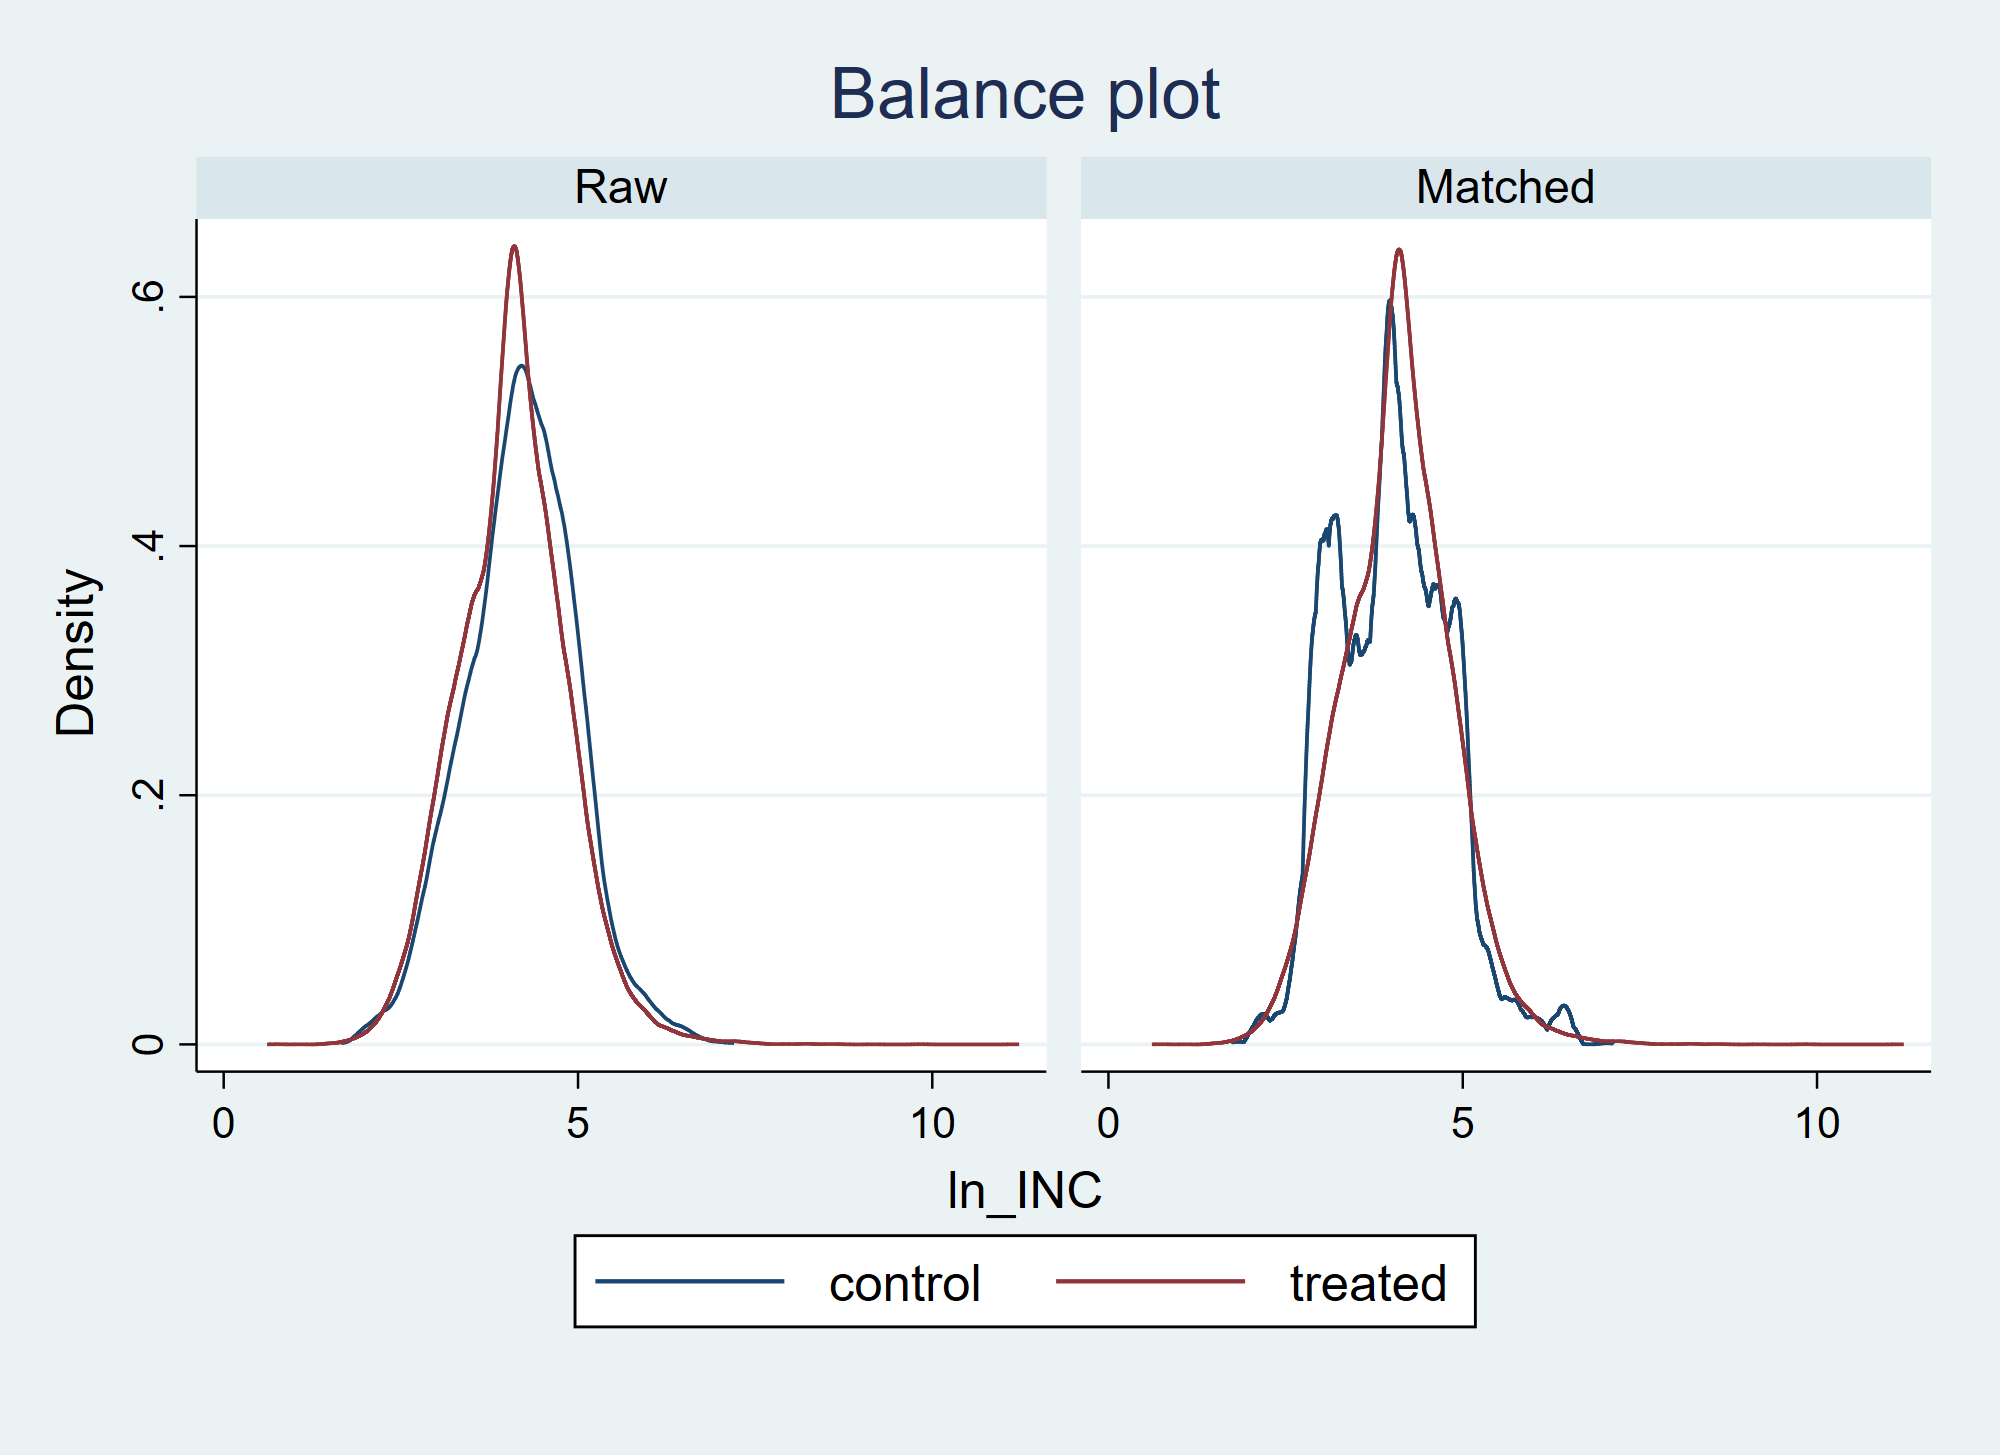
\includegraphics[width=0.8\textwidth]{figures/Figure3_Balance_Plot.png}
	\caption{Đánh giá chất lượng ghép cặp (Balance Plot) đối với biến Log Thu nhập}
	\label{fig:balance_plot}
\end{figure}

\subsubsection{Kiểm định biến công cụ}

Trong giai đoạn một của mô hình IV-2SLS, việc phải đồng thời công cụ hóa bốn biến nội sinh, bao gồm biến tham gia bảo hiểm y tế (BHYT) và các biến tương tác chéo, dẫn đến hiện tượng \textit{biến công cụ yếu một phần}. Điều này được phản ánh qua thống kê Kleibergen--Paap rk Wald $F = 2.77$, thấp hơn đáng kể so với ngưỡng quy tắc kinh nghiệm thường được sử dụng trong thực nghiệm ($F \geq 10$). Trong bối cảnh đó, các ước lượng IV tiêu chuẩn có thể tiềm ẩn rủi ro chệch. Tuy nhiên, sự nhất quán về chiều hướng tác động giữa kết quả IV-2SLS và phương pháp so khớp điểm xu hướng (PSM), vốn đã kiểm soát thiên lệch lựa chọn trên các biến quan sát, phần nào củng cố độ tin cậy của kết quả thực nghiệm. Do đó, các hệ số IV-2SLS trong nghiên cứu này chủ yếu được diễn giải theo chiều hướng tác động (dấu âm/dương), thay vì tập trung vào quy mô tuyệt đối của hệ số.  
Để tăng cường độ tin cậy của suy luận thống kê trong bối cảnh công cụ yếu, nghiên cứu tiếp tục thực hiện kiểm định Anderson--Rubin . Kết quả kiểm định Anderson--Rubin Wald cho thấy giá trị thống kê $F(4,62)=8.40$ với $p<0.001$, cho phép bác bỏ mạnh mẽ giả thuyết không ($H_0$) rằng các hệ số của nhóm biến nội sinh, bao gồm biến tham gia BHYT và các biến tương tác, đồng thời bằng không.
Do kiểm định Anderson--Rubin duy trì tính hợp lệ ngay cả khi các biến công cụ yếu, kết quả này cung cấp bằng chứng suy luận đáng tin cậy về sự tồn tại của tác động từ nhóm biến BHYT và các tương tác. Điều này củng cố tính vững của các phát hiện thực nghiệm, cho thấy rằng mặc dù mô hình phải xử lý cấu trúc nội sinh đa biến tương đối phức tạp, các kết quả về tác động phân hóa của bảo hiểm y tế, bao gồm hiệu ứng bảo vệ tài chính tại khu vực nông thôn và khả năng xuất hiện rủi ro đạo đức trong hành vi sử dụng dịch vụ y tế, vẫn duy trì tính ổn định và đáng tin cậy.


\clearpage
\subsection{Tổng hợp các kết quả}
Dựa trên chuỗi các phương pháp ước lượng kết hợp, nghiên cứu rút ra ba kết luận định lượng cốt lõi:

\begin{itemize}
	\item \textbf{Nghịch lý mở rộng chi phí:} Sở hữu thẻ BHYT không làm giảm tổng chi tiêu mà làm tăng mức OOP trung bình (khoảng $51.3\%$ theo PSM). BHYT đóng vai trò xúc tác, gỡ bỏ rào cản tài chính ban đầu để người dân tiếp cận dịch vụ thường xuyên hơn, kéo theo sự gia tăng tất yếu của đồng chi trả và thuốc men ngoài danh mục.
	
	\item \textbf{Sự phân hóa tác động không gian và rủi ro chéo:} Tại khu vực nông thôn, BHYT phát huy năng lực đệm giảm xóc cực tốt (hệ số $-1.147, p < 0.01$). Đặc biệt, đối phó với hành vi vượt tuyến, BHYT đóng vai trò là chiếc phanh hãm khẩn cấp tại đúng ngưỡng rủi ro thảm họa ($Q90$), cứu bệnh nhân khỏi phá sản y tế dù không triệt tiêu được hoàn toàn hình phạt tài chính.
	
	\item \textbf{Căn nguyên thể chế:} Gánh nặng tài chính tại Việt Nam không xuất phát từ việc thiếu độ phủ của BHYT, mà do cơ chế Phí dịch vụ đang dung túng cho việc tối đa hóa chi phí, trái ngược hoàn toàn với sự bảo vệ tốt hơn của mô hình Khoán định suất của BHYT tại Thái Lan.
	
	\item \textbf{Sự đánh đổi giữa hiệu quả và công bằng:} Mặc dù mô hình phân vị (SQREG) xác nhận BHYT có tác dụng giảm nhẹ rủi ro tại đuôi phân phối (Q90), sự tồn tại của hình phạt đồng chi trả khi vượt tuyến đang khoét sâu vào vấn đề bất bình đẳng y tế. Đứng từ góc độ định lý phúc lợi và nguyên tắc nhu cầu của Rawlsian, cơ chế hiện tại thiên về việc tối ưu hóa Hiệu quả (giảm tải tuyến trên bằng rào cản tài chính), nhưng lại hy sinh sự Công bằng. Việc chưa có cơ chế bảo vệ phân tầng khiến gánh nặng OOP mang tính lũy thoái; bệnh nhân nghèo ở nông thôn phải chịu tỷ lệ chi trả trên thu nhập cao hơn nhiều so với nhóm thu nhập cao ở thành thị khi đối mặt với cùng một cú sốc sức khỏe. Các phân tích sâu hơn bằng đường cong tập trung và chỉ số Gini về OOP sẽ là cần thiết để định lượng chính xác mức độ bất bình đẳng này.
\end{itemize}

\clearpage
\section{Kết luận và hàm ý chính sách}

Nghiên cứu này cung cấp bằng chứng thực nghiệm mạnh mẽ bác bỏ quan điểm truyền thống cho rằng việc tham gia BHYT luôn tỷ lệ thuận với việc giảm thiểu OOP. 
Thay vào đó, thông qua chiến lược phân tích hồi quy kết hợp dữ liệu cắt ngang VHLSS năm 2024 và dữ liệu mảng TVSEP (2007-2024) qua 9 làn sóng khảo sát, kết quả nghiên cứu cho thấy hệ thống BHYT tại Việt Nam đang vận hành theo một Hiệu ứng kép mang tính phi tuyến. 

Một mặt, dữ liệu VHLSS minh chứng rằng BHYT đóng vai trò như một chất xúc tác làm gia tăng tổng chi phí y tế (ATE tăng $51.3\%$), xuất phát từ việc khai thông nhu cầu khám chữa bệnh bị kìm nén và sự hiện diện của rủi ro đạo đức trong điều trị ngoại trú. Mặt mặt khác, tại ngưỡng rủi ro thảm họa ($Q90$), BHYT vẫn phát huy vai trò cơ chế giảm xóc tài chính cuối cùng, đặc biệt đối phó với nhóm bệnh nhân nông thôn buộc phải vượt tuyến. 

Tuy nhiên, giới hạn của sự bảo vệ này được bộc lộ rõ nét khi so sánh qua thời gian 17 năm với hệ thống Bao phủ toàn dân (UCS) của Thái Lan. Nghiên cứu phát hiện căn nguyên sâu xa khiến BHYT tại Việt Nam chưa thể nén rủi ro thảm họa một cách triệt để nằm ở khiếm khuyết trong thiết kế cơ chế BHYT. Cơ chế chi trả Phí dịch vụ mở kết hợp với sự bất cân xứng thông tin đã dung túng cho hiện tượng Cầu do nhà cung cấp tạo ra. Cơ sở y tế có động cơ lạm dụng chỉ định xét nghiệm và kỹ thuật cao vượt mức cần thiết để tối đa hóa doanh thu, trực tiếp đẩy người bệnh vào rủi ro thảm họa kép. Trong khi đó, mô hình Khoán định suất khép kín của Thái Lan đã chặn đứng được rủi ro này bằng cách chuyển giao gánh nặng chi phí về phía nhà cung cấp.

Từ những phát hiện định lượng cốt lõi trên, nghiên cứu đề xuất ba nhóm hàm ý chính sách chiến lược nhằm định hình lại quỹ đạo hướng tới Bao phủ Y tế Phổ quát (SDG 3.8) tại Việt Nam:

\begin{enumerate}
	\item \textbf{Đổi mới căn bản cơ chế thanh toán y tế (Kiểm soát SID):} Sự gia tăng chi phí bất thường ở các phân vị cao bắt nguồn từ rủi ro đạo đức của cả phía cung và phía cầu. Hệ thống BHYT cần đẩy nhanh lộ trình dịch chuyển từ phương thức thanh toán theo Phí dịch vụ (FFS) sang thanh toán theo Nhóm chẩn đoán (DRG) cho điều trị nội trú tuyến trên, và đặc biệt là áp dụng Khoán định suất cho mạng lưới y tế tuyến cơ sở. Cơ chế tài chính này sẽ triệt tiêu động cơ trục lợi từ hiện tượng Cầu do nhà cung cấp tạo ra (SID), buộc các bệnh viện phải tối ưu hóa chi phí thay vì lạm dụng chỉ định cận lâm sàng.
	
	\item \textbf{Đầu tư tuyến cơ sở:} Mức gia tăng chi phí đột biến từ hành vi vượt tuyến (hệ số $+2.039$ tại phân vị $Q90$) có thể được lý giải thông qua Mô hình Grossman. Người bệnh coi sức khỏe là một dạng vốn đầu tư và cân nhắc kỹ lưỡng chi phí thời gian. Sự thiếu hụt thuốc men và quy trình rườm rà tại y tế tuyến cơ sở đẩy chi phí thời gian lên quá cao, khiến người dân chấp nhận vượt tuyến, chịu phạt tiền để phục hồi sức khỏe nhanh hơn và sớm quay lại thị trường lao động. Do đó, thay vì thụ động dùng hình phạt đồng chi trả, chính sách BHYT cần chủ động mở rộng danh mục thuốc mãn tính và cắt giảm thời gian chờ đợi tại Trạm y tế xã. Đây là chìa khóa để giữ chân bệnh nhân dựa trên động cơ tối đa hóa hữu dụng.
	
	\item \textbf{Can thiệp từ phía Cầu (Nâng cao năng lực y tế cá nhân):} Cơ chế Capitation (phía Cung) sẽ không thể thành công toàn diện nếu bỏ qua các yếu tố quyết định hành vi từ phía Cầu. Theo Mô hình Grossman, trình độ học vấn và kiến thức y tế làm tăng hiệu suất sản xuất vốn sức khỏe. Do đó, thay vì chỉ tập trung vào tài chính y tế, Chính phủ cần đẩy mạnh các chương trình giáo dục sức khỏe cộng đồng, tư vấn dự phòng và nâng cao nhận thức về việc sử dụng thuốc không kê đơn (OTC) an toàn. Khi người dân được trang bị đủ kiến thức, họ sẽ tự điều chỉnh hành vi, giảm sự phụ thuộc không cần thiết vào hệ thống bệnh viện tuyến trên, từ đó tự nhiên tối ưu hóa chi phí cá nhân và giảm thiểu hành vi vượt tuyến phi lý.
	
	\item \textbf{Đảm bảo Công bằng theo chiều dọc cho nhóm yếu thế:} Mức phạt vượt tuyến hiện nay có thể mang lại Hiệu quả trong việc giảm tải tuyến trên, nhưng lại vi phạm nghiêm trọng nguyên tắc công bằng theo chiều dọc. Thực tế cho thấy, bệnh nhân nghèo ở nông thôn mắc bệnh hiểm nghèo thường không có lựa chọn nào khác ngoài việc cắn răng chịu phạt tài chính để giành giật sự sống, khiến rủi ro thảm họa dồn ép lên những người dễ tổn thương nhất. Do đó, Ngân sách Nhà nước không chỉ cần hỗ trợ 100\% mức đóng BHYT, mà còn phải thiết kế cơ chế miễn giảm hình phạt vượt tuyến cho các ca bạo bệnh đối với nhóm yếu thế, đảm bảo nguyên tắc an sinh: không một ai bị bỏ lại phía sau.
	
	\item \textbf{Sự cần thiết của phân tích phân nhóm:} Sự gia tăng chi phí ngoại trú chủ yếu được thúc đẩy bởi rủi ro đạo đức. Tuy nhiên, nếu giả định triệt tiêu hoàn toàn hành vi vượt tuyến, rủi ro đạo đức vẫn tồn tại nhưng biên độ gia tăng chi phí OOP sẽ được thu hẹp đáng kể. Điều này củng cố mạnh mẽ cho luận điểm Triết học Đạo đức  trong lĩnh vực y tế, bao gồm các mô hình vị lợi và bình đẳng dựa trên nhu cầu theo \textcite{hurley2000}: Việt Nam cần khẩn trương dịch chuyển trục chính sách từ mô hình vị lợi, vốn đang dung túng cho sự lãng phí nguồn lực thông qua vượt tuyến tràn lan, sang mô hình bình đẳng dựa trên Nhu cầu thông qua việc tái thiết lập Người gác cổng vững chắc tại tuyến cơ sở.

Lộ trình cải cách BHYT hướng tới năm 2030 được tóm tắt như sau:

\end{enumerate}

\begin{table}[htbp]
	\centering
	\renewcommand{\arraystretch}{1.3}
	\caption{Thang bậc Chính sách: Lộ trình cải cách BHYT hướng tới năm 2030}
	\label{tab:policy_ladder}
	\resizebox{\textwidth}{!}{
		\begin{tabular}{p{4cm} p{4.5cm} p{4.5cm} p{4.5cm}}
			\toprule
			\textbf{Tiêu chí cốt lõi} & \textbf{Việt Nam (Hiện tại)} & \textbf{Thái Lan (Tham chiếu UCS)} & \textbf{Đề xuất cho VN (Tầm nhìn đến 2030)} \\
			\midrule
			\textbf{Cơ chế thanh toán} (Phía Cung) & Phí dịch vụ. Tạo động lực lạm dụng chỉ định (SID). & Khoán định suất và DRG. Chuyển rủi ro sang cơ sở y tế. & Áp dụng Khoán định suất cho y tế cơ sở và DRG cho điều trị nội trú tuyến trên \\
			\addlinespace
			\textbf{Hệ thống Gác cổng} & Lỏng lẻo. Chủ yếu dùng hình phạt tài chính (đồng chi trả) để cản bước. & Nghiêm ngặt. Đăng ký cố định tại tuyến chăm sóc ban đầu & Đầu tư thực chất cho tuyến xã (mở rộng danh mục thuốc mãn tính) để giữ chân bệnh nhân tự nguyện. \\
			\addlinespace
			\textbf{Triết lý Công bằng} & Vị lợi: Tối đa hóa khả năng tiếp cận y tế cơ bản cho số đông. & Bình đẳng: Xóa bỏ rào cản tài chính tại điểm sử dụng dịch vụ. & Công bằng theo chiều dọc: Miễn trừ hình phạt vượt tuyến cho nhóm yếu thế mắc bạo bệnh. \\
			\bottomrule
		\end{tabular}
	}
\end{table}

\clearpage
\section{Giới hạn của nghiên cứu và hướng phát triển} 

Nghiên cứu áp dụng một hệ thống các kỹ thuật nhận diện nhân quả và kiểm định độ vững (IV-2SLS, PSM, SQREG, RIF-TWFE), vẫn tồn tại một số hạn chế khách quan nhất định như sau:

\textit{Thứ nhất, về đặc tính dữ liệu vi mô:} Cả hai bộ khảo sát VHLSS và TVSEP đều phụ thuộc vào recall bias của hộ gia đình đối với các khoản chi tiêu y tế trong 12 tháng qua, có thể dẫn đến sai số đo lường nhất định. Thêm vào đó, việc duy trì theo dõi các hộ gia đình xuyên suốt 17 năm trong tập dữ liệu mảng (TVSEP) không thể tránh khỏi hiện tượng hao hụt mẫu do các nguyên nhân nhân khẩu học như di cư hoặc tách/nhập hộ. Ngoài ra, dữ liệu mảng TVSEP đại diện cho khu vực nông thôn của hai quốc gia. Do đó, phát hiện về năng lực vượt trội của mô hình Khoán định suất (Thái Lan) so với Phí dịch vụ (Việt Nam) mang tính phản ánh cho nhóm yếu thế tại nông thôn, nơi cấu trúc y tế cơ sở đóng vai trò là lưới an sinh trọng yếu nhất.

\textit{Thứ hai, về khuyết thiếu các biến số phía cung:} Mô hình hiện tại chủ yếu khai thác các đặc điểm từ phía cầu (hộ gia đình). Các yếu tố định hình quyết định khám chữa bệnh từ phía cung như: khoảng cách vật lý chính xác từ nhà đến bệnh viện, mật độ giường bệnh, hay chất lượng trang thiết bị y tế của từng địa phương... chỉ mới được hấp thụ một cách gián tiếp thông qua các hiệu ứng cố định cấp tỉnh.

\textit{Thứ ba, về dạng hàm toán học của biến phụ thuộc:} Do bản chất của chi tiêu y tế (OOP) thường chứa một tỷ lệ đáng kể các giá trị bằng $0$ (nhóm hộ gia đình không phát sinh ốm đau trong kỳ khảo sát), việc sử dụng phép biến đổi logarit $\ln(OOP+1)$ có thể chưa nắm bắt trọn vẹn đặc tính của dữ liệu gốc. Các nghiên cứu tiếp theo sẽ triển khai thêm các Sensitivity Test sử dụng mô hình Tobit hoặc mô hình Hai bước của Heckman để xử lý triệt để hiện tượng tập trugng dữ liệu tại điểm không, qua đó tinh chỉnh độ chính xác của các ước lượng hệ số tác động biên.

Trong tương lai, các nghiên cứu tiếp nối có thể khắc phục những giới hạn này thông qua hai hướng tiếp cận mới. Một là, ứng dụng phương pháp Kinh tế lượng không gian để lượng hóa chính xác chi phí di chuyển và độ co giãn của cầu y tế theo không gian địa lý. Hai là, tiến hành liên kết dữ liệu giữa bộ vi dữ liệu khảo sát hộ gia đình với dữ liệu hành chính từ Hệ thống Thông tin Y tế Quốc gia (DHIS2) hoặc cơ sở dữ liệu thanh toán bồi thường của cơ quan Bảo hiểm Xã hội. Sự kết hợp này sẽ cung cấp một lăng kính toàn cảnh và chính xác tuyệt đối về tương tác vi mô giữa cấu trúc cung y tế và hành vi người bệnh.

%====================================================
% APPENDIX 
%====================================================
\newpage
\appendix
\section{Phụ lục}

 % ---------------------------------------------------
% PHẦN I: DỮ LIỆU VÀ KẾT QUẢ TỪ VHLSS 2024
% ---------------------------------------------------
\subsection{Phân tích VHLSS 2024}

\subsubsection{Phụ lục A.1 – Thống kê mô tả các biến số chính (VHLSS)}

\begin{table}[htbp]
	\centering
	\caption{Thống kê mô tả các biến trong mô hình VHLSS ($N = 46.995$)}
	\label{tab:summary_stats_vhlss}
	\begin{tabular}{lcccc}
		\toprule
		\textbf{Biến số} & \textbf{Trung bình} & \textbf{Độ lệch chuẩn} & \textbf{Giá trị Min} & \textbf{Giá trị Max} \\
		\midrule
		\multicolumn{5}{l}{\textit{\textbf{Biến phụ thuộc (Chi phí y tế)}}} \\
		Tổng chi phí OOP (Triệu VND) & 5.578 & 13.040 & 0 & 660 \\
		Chi phí OOP Nội trú (Triệu VND) & 1.495 & 10.278 & 0 & 600 \\
		Chi phí OOP Ngoại trú (Triệu VND) & 1.341 & 5.141 & 0 & 324 \\
		\addlinespace
		\multicolumn{5}{l}{\textit{\textbf{Biến độc lập chính và Đặc điểm hộ gia đình}}} \\
		Bảo hiểm y tế ($INS\_DUMMY$: 1=Có) & 0.971 & 0.168 & 0 & 1 \\
		Hành vi vượt tuyến ($BYPASSED$: 1=Có) & 0.375 & 0.484 & 0 & 1 \\
		Khu vực Nông thôn ($RURAL$: 1=Có) & 0.603 & 0.489 & 0 & 1 \\
		Log thu nhập bình quân ($\ln\_INC$) & 4.162 & 0.752 & 0.697 & 11.149 \\
		Tuổi chủ hộ ($AGE\_HEAD$) & 53.945 & 13.675 & 10 & 106 \\
		Giới tính chủ hộ ($SEX\_HEAD$: 1=Nam) & 0.700 & 0.458 & 0 & 1 \\
		Quy mô hộ gia đình ($HH\_SIZE$) & 3.513 & 1.646 & 1 & 16 \\
		\addlinespace
		\multicolumn{5}{l}{\textit{\textbf{Biến công cụ (Instrumental Variable)}}} \\
		Tỷ lệ BHYT cấp xã ($IV\_COMMUNE$) & 0.925 & 0.100 & 0.026 & 1 \\
		\bottomrule
	\end{tabular}
	\vspace{0.15cm}
	
	\parbox{14cm}{\footnotesize \textit{Ghi chú:} Thống kê mô tả đã áp dụng trọng số mẫu (sample weights) của VHLSS 2024.}
\end{table}

\newpage
\subsubsection{Phụ lục B.1 – Kết quả mô hình biến công cụ (IV-2SLS phân rã OOP)}

\begin{table}[htbp]
	\centering
	\def\sym#1{\ifmmode^{#1}\else\(^{#1}\)\fi}
	\caption{Tác động của BHYT lên cấu trúc chi phí OOP (Mô hình IV-2SLS)}
	\label{tab:iv_appendix}
	\begin{tabular}{lccc}
		\toprule
		&\textbf{(1)}&\textbf{(2)}&\textbf{(3)}\\
		\textbf{Biến độc lập}&\textbf{Log(Tổng OOP)}&\textbf{Log(OOP Nội trú)}&\textbf{Log(OOP Ngoại trú)}\\
		\midrule
		BHYT (Cơ sở) & 1.256\sym{***} & -0.219 & 0.292\sym{*} \\
		& (0.177) & (0.155) & (0.157) \\
		\addlinespace
		BHYT $\times$ Nông thôn & -0.967\sym{***} & -0.115 & 0.035 \\
		& (0.286) & (0.178) & (0.137) \\
		\addlinespace
		BHYT $\times$ Vượt tuyến & 2.413 & 2.806 & 0.405 \\
		& (1.833) & (2.172) & (1.513) \\
		\addlinespace
		BHYT $\times$ Nông thôn $\times$ Vượt tuyến & -3.533 & -1.345 & -2.971\sym{*} \\
		& (2.151) & (2.431) & (1.707) \\
		\addlinespace
		Nông thôn (Base) & 0.850\sym{***} & 0.083 & -0.026 \\
		& (0.262) & (0.155) & (0.133) \\
		\addlinespace
		Vượt tuyến (Base) & -1.648 & -2.244 & 0.443 \\
		& (1.795) & (2.092) & (1.493) \\
		\midrule
		Biến kiểm soát ($X$) & Có & Có & Có \\
		Fixed Effects (Tỉnh) & Có & Có & Có \\
		\midrule
		Số quan sát ($N$) & 46.995 & 46.995 & 46.995 \\
		\bottomrule
		\multicolumn{4}{p{13cm}}{\footnotesize \textit{Ghi chú:} Sai số chuẩn vững (Robust clustered SEs) theo cấp tỉnh đặt trong ngoặc đơn. \sym{*} \(p<0.10\), \sym{**} \(p<0.05\), \sym{***} \(p<0.01\)}
	\end{tabular}
\end{table}

\newpage
\subsubsection{Phụ lục C.1 – Kết quả hồi quy Phân vị đồng thời (SQREG)}

\begin{table}[htbp]
	\centering
	\def\sym#1{\ifmmode^{#1}\else\(^{#1}\)\fi}
	\caption{Tác động của BHYT dọc theo phân phối chi phí (Mô hình SQREG - VHLSS)}
	\label{tab:sqreg_appendix}
	\begin{tabular}{lcccc}
		\toprule
		&\textbf{(1)}&\textbf{(2)}&\textbf{(3)}&\textbf{(4)}\\
		\textbf{Biến độc lập}&\textbf{Q25}&\textbf{Q50}&\textbf{Q75}&\textbf{Q90}\\
		\midrule
		BHYT (Cơ sở) & 0.585\sym{***} & 0.681\sym{***} & 0.669\sym{***} & 0.675\sym{***} \\
		& (0.025) & (0.023) & (0.033) & (0.043) \\
		\addlinespace
		Vượt tuyến & 0.558\sym{***} & 0.916\sym{***} & 1.654\sym{***} & 2.039\sym{***} \\
		& (0.081) & (0.088) & (0.121) & (0.228) \\
		\addlinespace
		BHYT $\times$ Nông thôn & -0.198\sym{***} & -0.073\sym{***} & 0.014 & -0.011 \\
		& (0.030) & (0.024) & (0.041) & (0.064) \\
		\addlinespace
		BHYT $\times$ Vượt tuyến & -0.045 & -0.290\sym{***} & -0.643\sym{***} & -0.605\sym{***} \\
		& (0.083) & (0.090) & (0.125) & (0.228) \\
		\addlinespace
		BHYT $\times$ Nông thôn $\times$ Vượt tuyến & 0.170\sym{***} & 0.079\sym{***} & 0.055\sym{**} & 0.044 \\
		& (0.019) & (0.017) & (0.025) & (0.031) \\
		\midrule
		Biến kiểm soát nhân khẩu học & Có & Có & Có & Có \\
		Pseudo $R^2$ & 0.202 & 0.209 & 0.260 & 0.314 \\
		Số quan sát ($N$) & 46.995 & 46.995 & 46.995 & 46.995 \\
		\bottomrule
		\multicolumn{5}{p{13.5cm}}{\footnotesize \textit{Ghi chú:} Mô hình Hồi quy phân vị đồng thời với 100 lần bootstrap. \sym{***} \(p<0.01\)}
	\end{tabular}
\end{table}

\newpage
\subsubsection{Phụ lục D.1 - Ma trận tương quan và Kiểm định Đa cộng tuyến}



\begin{table}[htbp]
	\centering
	\caption{Ma trận tương quan có trọng số (VHLSS)}
	\label{tab:corr_matrix}
	\resizebox{\textwidth}{!}{%
		\begin{tabular}{lcccccccc}
			\toprule
			\textbf{Biến số} & \textbf{ln\_OOP} & \textbf{INS} & \textbf{RURAL} & \textbf{BYP} & \textbf{ln\_INC} & \textbf{AGE} & \textbf{SEX} & \textbf{HH\_SIZE} \\
			\midrule
			\texttt{ln\_OOP} & 1.000 & & & & & & & \\
			\texttt{INS\_DUMMY} & 0.187 & 1.000 & & & & & & \\
			\texttt{RURAL} & -0.063 & 0.016 & 1.000 & & & & & \\
			\texttt{BYPASSED} & 0.509 & 0.092 & -0.078 & 1.000 & & & & \\
			\texttt{ln\_INC} & 0.129 & -0.029 & -0.264 & 0.001 & 1.000 & & & \\
			\texttt{AGE\_HEAD} & 0.094 & 0.038 & 0.028 & 0.153 & -0.125 & 1.000 & & \\
			\texttt{SEX\_HEAD} & 0.059 & 0.015 & 0.125 & -0.029 & 0.014 & -0.143 & 1.000 & \\
			\texttt{HH\_SIZE} & 0.284 & 0.141 & 0.049 & 0.055 & -0.139 & -0.141 & 0.214 & 1.000 \\
			\bottomrule
		\end{tabular}%
	}
\end{table}

\textit{Ghi chú VIF:} Kiểm định Hệ số phóng đại phương sai (VIF) cho mô hình cơ sở đạt mức trung bình là \textbf{4.14}, thấp hơn nhiều so với ngưỡng cảnh báo 10, chứng tỏ mô hình không vi phạm giả định đa cộng tuyến nghiêm trọng.

\newpage

\subsubsection{Phụ lục E.1 – Chẩn đoán khuyết tật mô hình và Sức mạnh Biến công cụ}

\begin{table}[htbp]
	\centering
	\caption{Kiểm định chẩn đoán mô hình IV-2SLS}
	\label{tab:diagnostics}
	\begin{tabular}{llcc}
		\toprule
		\textbf{Loại kiểm định} & \textbf{Thống kê / Hệ số} & \textbf{Giá trị} & \textbf{P-value} \\
		\midrule
		\multicolumn{4}{l}{\textbf{Panel A: Sức mạnh Biến công cụ (First-stage)}} \\
		F-test (\texttt{INS\_DUMMY}) & Thống kê SW F-test & 96.65 & 0.000 \\
		F-test (\texttt{ins\_rural\_vuot}) & Thống kê SW F-test & 534.43 & 0.000 \\
		\midrule
		\multicolumn{4}{l}{\textbf{Panel B: Kiểm định phương sai sai số thay đổi (Heteroskedasticity)}} \\
		Kiểm định Pagan-Hall & Thống kê $\chi^2(8)$ & 2982.26 & 0.000 \\
		\midrule
		\multicolumn{4}{l}{\textbf{Panel C: Tương quan nội cụm (Intra-cluster correlation)}} \\
		Hệ số ICC (Cấp Tỉnh) & Giá trị ICC & 0.0706 & - \\
		\bottomrule
	\end{tabular}
\end{table}


Bảng~\ref{tab:iv_diagnostics} trình bày chi tiết các kiểm định liên quan đến mô hình biến công cụ, bao gồm kiểm định underidentification, weak instrument và Anderson--Rubin.

\begin{table}[H]
	\centering
	\caption{Kiểm định biến công cụ trong mô hình IV-2SLS}
	\label{tab:iv_diagnostics}
	\begin{tabular}{lcc}
		\hline
		\textbf{Kiểm định} & \textbf{Thống kê} & \textbf{Kết quả} \\
		\hline
		Kleibergen--Paap rk LM test & $\chi^2 = 7.657$ & $p = 0.0057$ \\
		Kleibergen--Paap rk Wald F & $F = 2.77$ & Weak instrument \\
		Anderson--Rubin Wald test & $F(4,62)=8.40$ & $p < 0.001$ \\
		\hline
	\end{tabular}
	
	\begin{flushleft}
		\footnotesize
		\textit{Ghi chú:} Bảng trình bày các kiểm định chẩn đoán cho mô hình IV-2SLS. Thống kê Kleibergen--Paap rk Wald $F$ thấp cho thấy khả năng tồn tại biến công cụ yếu. Tuy nhiên, kiểm định Anderson--Rubin cung cấp suy luận vững trong bối cảnh công cụ yếu.
	\end{flushleft}
	
\end{table}

% ---------------------------------------------------
% PHẦN II: DỮ LIỆU VÀ KẾT QUẢ TỪ TVSEP (PANEL)
% ---------------------------------------------------
\newpage
\subsection{Phân tích so sánh với Thái Lan ( qua dữ liệu TVSEP 2007-2024)}

\subsubsection{Phụ lục A.2 – Thống kê mô tả dữ liệu mảng TVSEP (Phân tách theo Quốc gia và BHYT)}

Dựa trên kết quả thống kê mô tả từ tập dữ liệu gộp, bảng dưới đây trình bày các đặc điểm mẫu quan sát, phân tách rõ ràng sự khác biệt giữa các hộ gia đình có và không có Bảo hiểm Y tế tại hai quốc gia trong suốt 17 năm.

\begin{table}[htbp]
	\centering
	\caption{Thống kê mô tả các biến số chính trong mô hình TVSEP ($N = 31.779$)}
	\label{tab:summary_stats_tvsep_detail}
	\resizebox{\textwidth}{!}{
		\begin{tabular}{lcccccccc}
			\toprule
			& \multicolumn{2}{c}{\textbf{Việt Nam (Không BHYT)}} & \multicolumn{2}{c}{\textbf{Việt Nam (Có BHYT)}} & \multicolumn{2}{c}{\textbf{Thái Lan (Không BHYT)}} & \multicolumn{2}{c}{\textbf{Thái Lan (Có BHYT)}} \\
			\cmidrule(lr){2-3} \cmidrule(lr){4-5} \cmidrule(lr){6-7} \cmidrule(lr){8-9}
			\textbf{Biến số} & \textbf{Mean} & \textbf{SD} & \textbf{Mean} & \textbf{SD} & \textbf{Mean} & \textbf{SD} & \textbf{Mean} & \textbf{SD} \\
			\midrule
			Log(OOP PPP USD Real) & 6.215 & 2.211 & 3.984 & 2.720 & 6.266 & 2.443 & 3.410 & 2.895 \\
			Quy mô hộ gia đình (người) & 4.988 & 2.031 & 5.271 & 2.031 & 5.198 & 2.209 & 5.759 & 2.106 \\
			Tuổi chủ hộ (năm) & 48.072 & 15.181 & 55.755 & 12.565 & 51.804 & 14.681 & 61.553 & 13.556 \\
			Giới tính chủ hộ (1 = Nam) & 0.143 & 0.350 & 0.413 & 0.493 & 0.192 & 0.394 & 0.374 & 0.484 \\
			Cú sốc sức khỏe (1 = Có) & 0.089 & 0.285 & 0.114 & 0.318 & 0.063 & 0.242 & 0.059 & 0.236 \\
			\midrule
			\textbf{Số quan sát ($N$)} & \multicolumn{2}{c}{14.052} & \multicolumn{2}{c}{1.769} & \multicolumn{2}{c}{13.829} & \multicolumn{2}{c}{2.129} \\
			\bottomrule
		\end{tabular}
	}
	\vspace{1ex}
	\parbox{\textwidth}{\footnotesize \textit{Ghi chú:} Trích xuất từ dữ liệu mảng TVSEP (2007-2024). Chi phí y tế (OOP) đã được điều chỉnh lạm phát (năm gốc 2010) và quy đổi sang USD theo Ngang giá sức mua (PPP) để đảm bảo tính so sánh xuyên quốc gia. Dữ liệu cho thấy nhóm có BHYT ở cả hai nước có mức chi OOP trung bình thấp hơn, nhưng độ phân tán rủi ro (SD) lại cao hơn nhóm không có BHYT.}
\end{table}

\newpage
\subsubsection{Phụ lục B.2 – Kết quả Hồi quy Hiệu ứng cố định (TWFE) và Phân vị (SQREG)}

Bảng dưới đây trình bày kết quả hồi quy chi tiết, đối chiếu giữa mức trung bình (TWFE) và ngưỡng thảm họa y tế (Phân vị thứ 90 - SQREG) nhằm kiểm chứng cơ chế điều tiết của hành vi vượt tuyến giữa hai hệ thống thể chế.

\begin{table}[htbp]
	\centering
	\def\sym#1{\ifmmode^{#1}\else\(^{#1}\)\fi}
	\renewcommand{\arraystretch}{1.15} % Giãn cách dòng cho thoáng mắt
	\caption{Tác động của BHYT và Hành vi Vượt tuyến đến Chi tiêu y tế (Việt Nam vs Thái Lan)}
	\label{tab:results_tvsep}
	\resizebox{\textwidth}{!}{
		\begin{tabular}{lccc}
			\toprule
			&\textbf{(1)}&\textbf{(2)}&\textbf{(3)}\\
			\textbf{Biến độc lập}&\textbf{TWFE Baseline (Mean)}&\textbf{TWFE Mechanism (Mean)}&\textbf{SQREG ($Q90$ - Thảm họa)}\\
			\midrule
			\textbf{BHYT (Chung - Đại diện VN)} & -0.077 & -0.073 & 0.345\sym{***} \\
			& (0.065) & (0.065) & (0.043) \\
			\addlinespace
			\textbf{BHYT $\times$ Thái Lan (Hiệu ứng chênh lệch)} & 0.554\sym{***} & 0.546\sym{***} & -0.452\sym{***} \\
			& (0.085) & (0.085) & (0.055) \\
			\addlinespace
			\textbf{Vượt tuyến (Chung - Đại diện VN)} & & 0.065\sym{***} & -0.166\sym{***} \\
			& & (0.023) & (0.024) \\
			\addlinespace
			\textbf{Vượt tuyến $\times$ Thái Lan (Hiệu ứng gác cổng)} & & 0.014 & 0.244\sym{***} \\
			& & (0.030) & (0.033) \\
			\addlinespace
			Cú sốc sức khỏe & 0.078\sym{***} & 0.065\sym{***} & 0.096\sym{***} \\
			& (0.022) & (0.021) & (0.032) \\
			\addlinespace
			Quy mô hộ gia đình & 0.091\sym{***} & 0.090\sym{***} & 0.052\sym{***} \\
			& (0.007) & (0.007) & (0.004) \\
			\midrule
			Kiểm soát Đặc điểm Hộ gia đình ($X$) & Có & Có & Có \\
			Cố định hiệu ứng Hộ gia đình ($\mu_i$) & Có & Có & Không (Khử đa cộng tuyến) \\
			Cố định hiệu ứng Năm khảo sát ($\lambda_t$) & Có & Có & Có \\
			\midrule
			Số quan sát ($N$) & 23.754\textsuperscript{a} & 23.754\textsuperscript{a} & 29.473 \\
			$R^2$ / Pseudo $R^2$ & 0.836 & 0.836 & 0.358 \\
			\bottomrule
			\multicolumn{4}{p{16cm}}{\footnotesize \textit{Ghi chú:} Cột (1) và (2) sử dụng mô hình Hiệu ứng cố định hai chiều (HDFE) với sai số chuẩn vững được san cụm theo cấp Thôn (village) đặt trong ngoặc đơn. Cột (3) sử dụng mô hình Hồi quy phân vị đồng thời tại ngưỡng $Q90$ với sai số chuẩn Bootstrap. Mô hình phân vị không áp dụng Fixed Effect cấp hộ gia đình để tránh vấn đề tham số ngẫu nhiên (incidental parameters problem). \newline 
				\textsuperscript{a} \textit{Số lượng quan sát trong mô hình TWFE giảm xuống còn $23.754$ do thuật toán tự động loại bỏ các quan sát đơn lẻ (singleton observations) không đóng góp vào phương sai nội nhóm (within-variance) theo thời gian.} \newline
				\sym{*} \(p<0.10\), \sym{**} \(p<0.05\), \sym{***} \(p<0.01\)}
		\end{tabular}
	}
\end{table}

\clearpage
\subsubsection{Phụ lục C.2 – Kết quả Phân tích Động học Thời gian}

Bảng dưới đây trích xuất các hệ số tương tác 3 chiều ($\text{INS\_dummy} \times \text{THAI\_dummy} \times \text{wave}$) từ mô hình Event-study nhằm kiểm chứng quỹ đạo tác động của BHYT tại Thái Lan so với Việt Nam qua các làn sóng khảo sát.

\begin{table}[htbp]
	\centering
	\def\sym#1{\ifmmode^{#1}\else\(^{#1}\)\fi}
	\caption{Hệ số tác động động học của BHYT Thái Lan qua các năm}
	\label{tab:event_study_tvsep}
	\begin{tabular}{lcccc}
		\toprule
		\textbf{Làn sóng (Wave)} & \textbf{Hệ số Beta} & \textbf{Sai số chuẩn} & \textbf{Thống kê $t$} & \textbf{P-value} \\
		\midrule
		Wave 2008 & 1.571\sym{***} & 0.282 & 5.57 & 0.000 \\
		Wave 2010 & 1.043\sym{***} & 0.262 & 3.98 & 0.000 \\
		Wave 2011 & 0.658\sym{**} & 0.309 & 2.13 & 0.034 \\
		Wave 2013 & 0.885\sym{***} & 0.300 & 2.95 & 0.003 \\
		Wave 2016 & 0.913\sym{***} & 0.314 & 2.91 & 0.004 \\
		Wave 2017 & 0.907\sym{***} & 0.301 & 3.01 & 0.003 \\
		\bottomrule
		\multicolumn{5}{p{13cm}}{\footnotesize \textit{Ghi chú:} Năm cơ sở (Base year) là Wave 2007. Sự tồn tại của các hệ số có ý nghĩa thống kê dương mạnh mẽ chứng tỏ cấu trúc thể chế của Thái Lan duy trì quỹ đạo tác động ổn định kéo dài suốt nhiều năm, không bị nhiễu bởi các cú sốc vĩ mô ngắn hạn. \sym{**} \(p<0.05\), \sym{***} \(p<0.01\)}
	\end{tabular}
\end{table}
	
%====================================================
% REFERENCES
%====================================================
\clearpage
\section*{Tài liệu tham khảo}
\addcontentsline{toc}{section}{Tài liệu tham khảo}
\printbibliography[heading=none, title={}]
\renewcommand{\bibfont}{\small}
\end{document}